\chapter*{Cusco et la vallée sacrée des Incas\markboth{Cusco et la vallée sacrée des Incas}{}}
\section*{31 mai 2015}

À Cusco je reste à l'auberge \og Estrellitas \fg qui est quasiment la casa de ciclistas de la ville : la plupart des cyclistes qui passent sont ici. J'y ai même croisé une famille voyageant en tandem avec 2 enfants. 
\begin{center} 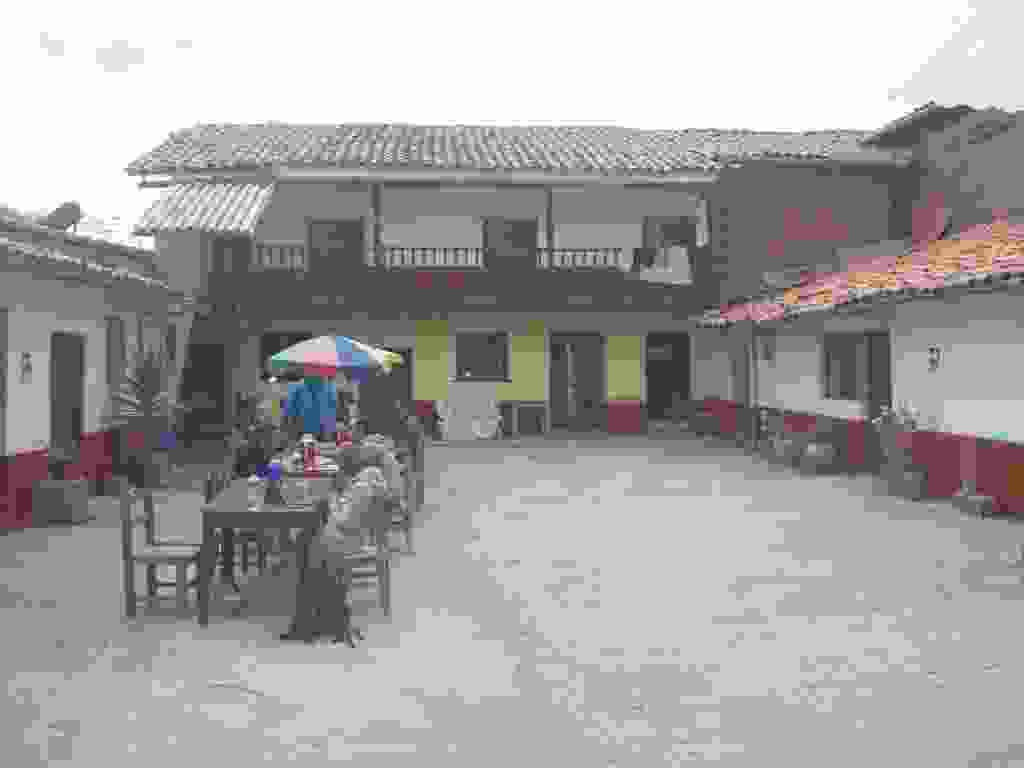
\includegraphics[width=\mywidth]{../wp-content/uploads/2015/05/P5294564-1024x768.jpg} \end{center}
\vspace{-\topsep}
\pagebreak

Cusco est une ville très touristique qui fût la capitale de l'empire Inca. 
\begin{center} 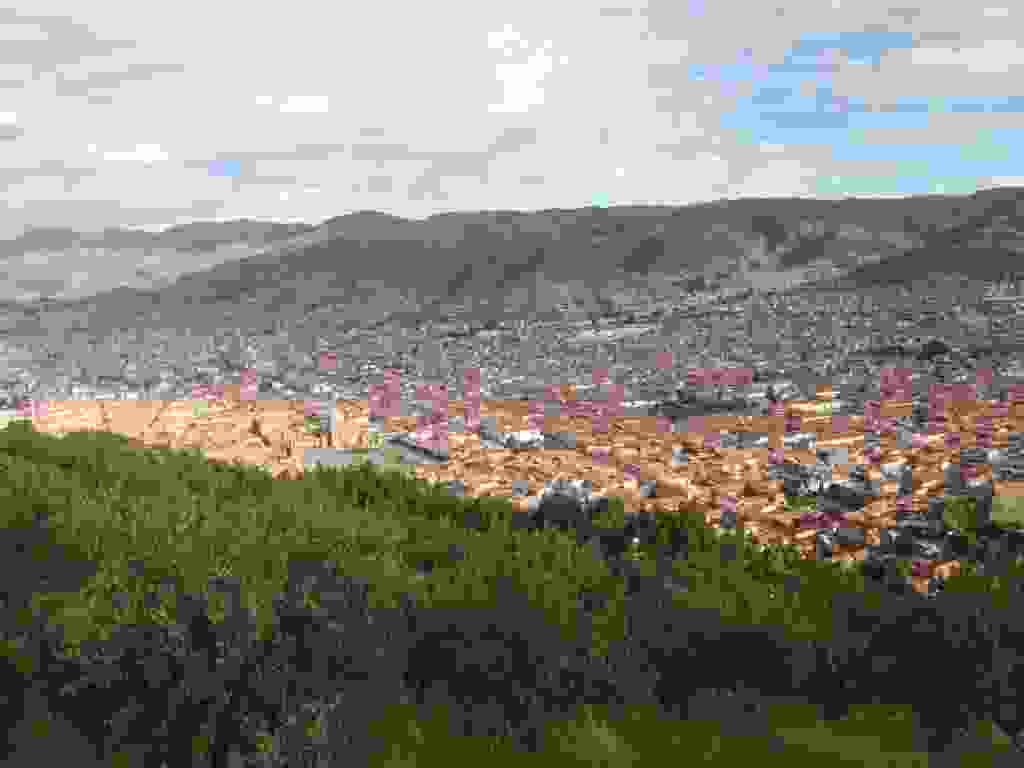
\includegraphics[width=\mywidth]{../wp-content/uploads/2015/05/P5174144-1024x768.jpg} \end{center}

Les rues du centre historique de style colonial. 
\begin{center} 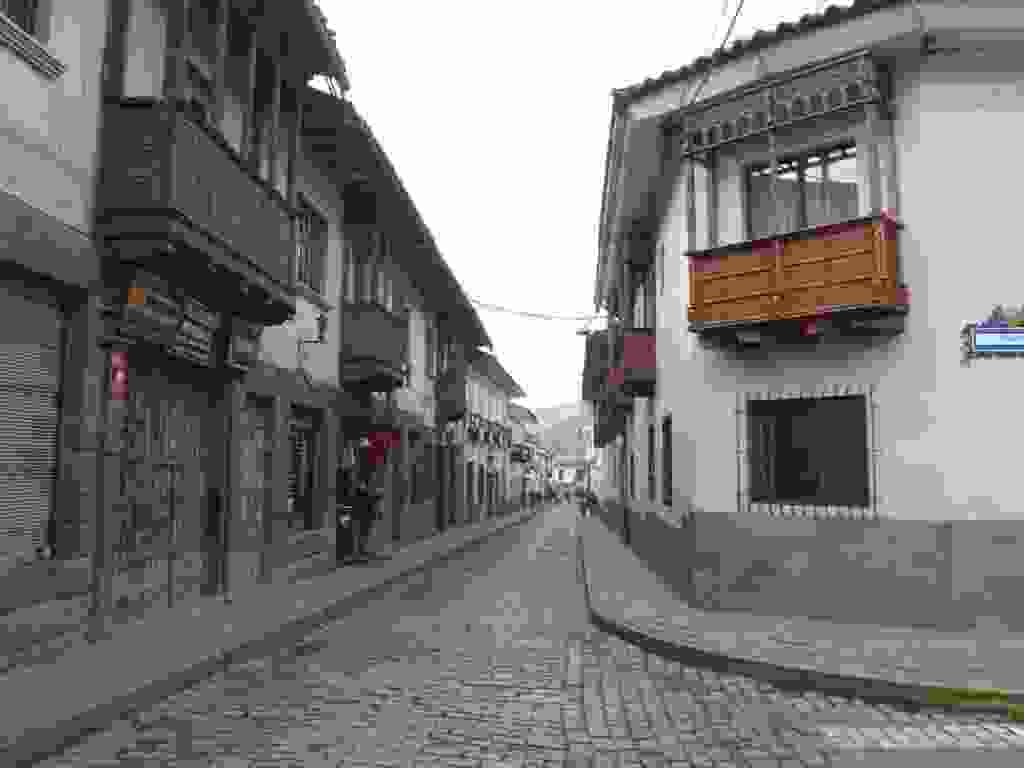
\includegraphics[width=\mywidth]{../wp-content/uploads/2015/05/P5174112-1024x768.jpg} \end{center}
\vspace{-\topsep}
\pagebreak
~
\begin{center} 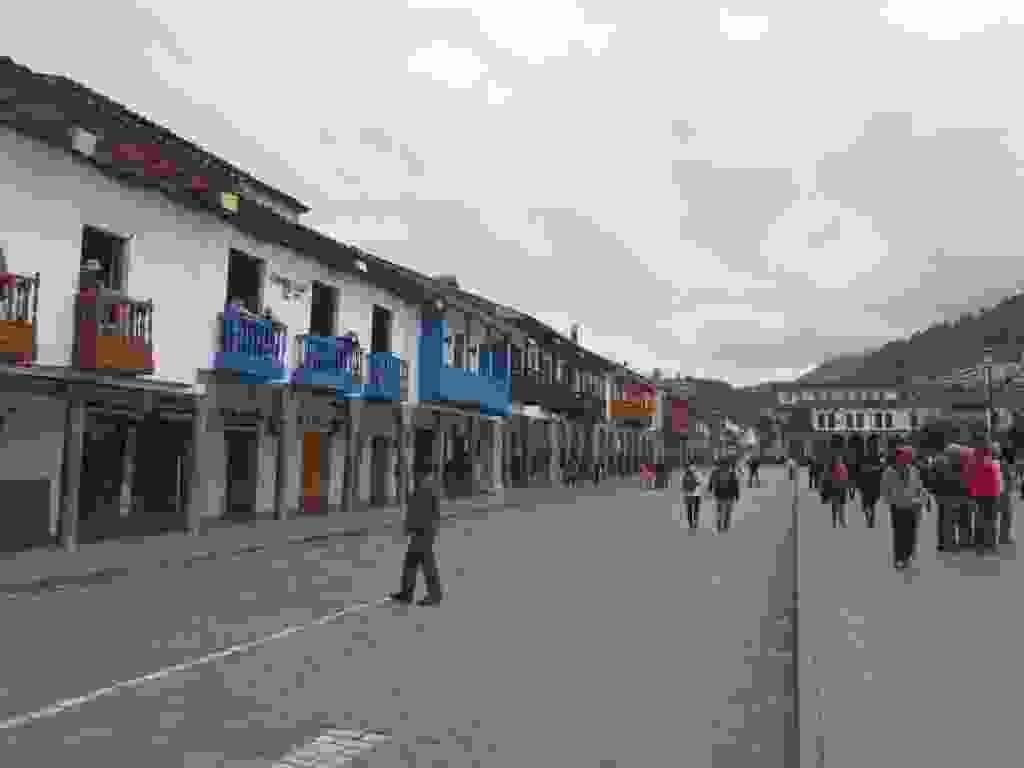
\includegraphics[width=\mywidth]{../wp-content/uploads/2015/05/P5174120-1024x768.jpg} \end{center}
~
\begin{center} 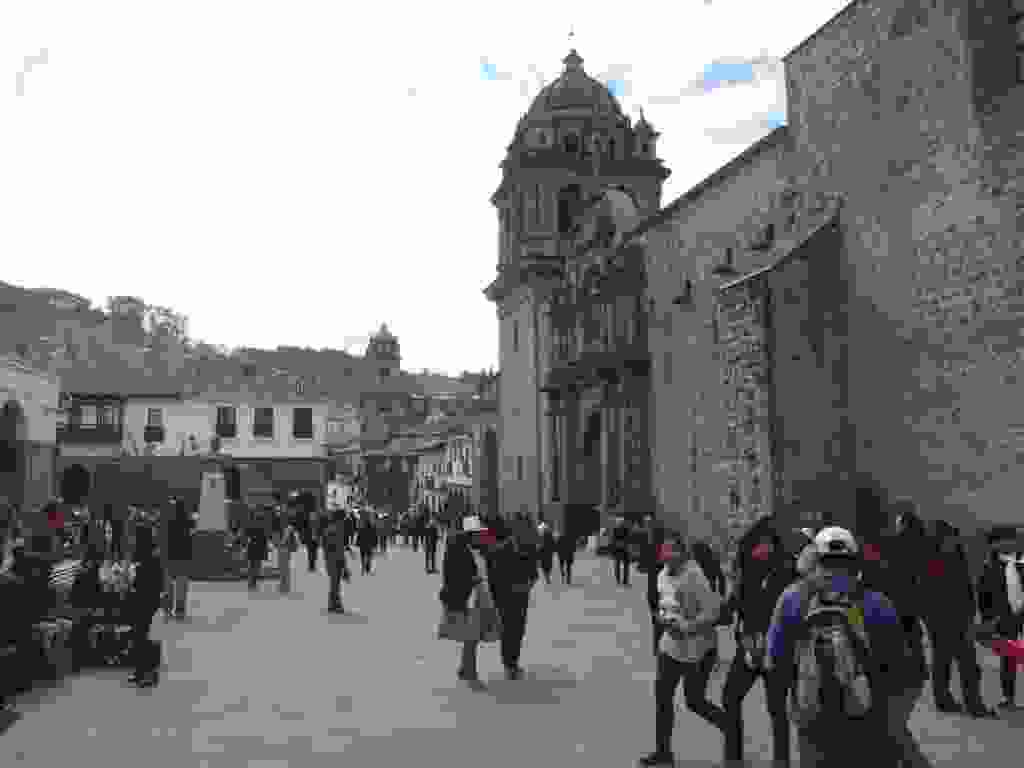
\includegraphics[width=\mywidth]{../wp-content/uploads/2015/05/P5174121-1024x768.jpg} \end{center}
\vspace{-\topsep}
%\vspace{-0.75mm}
\pagebreak

Il y avait un défilé sur la Plaza de Armas le jour où je suis arrivé. 
\begin{center} 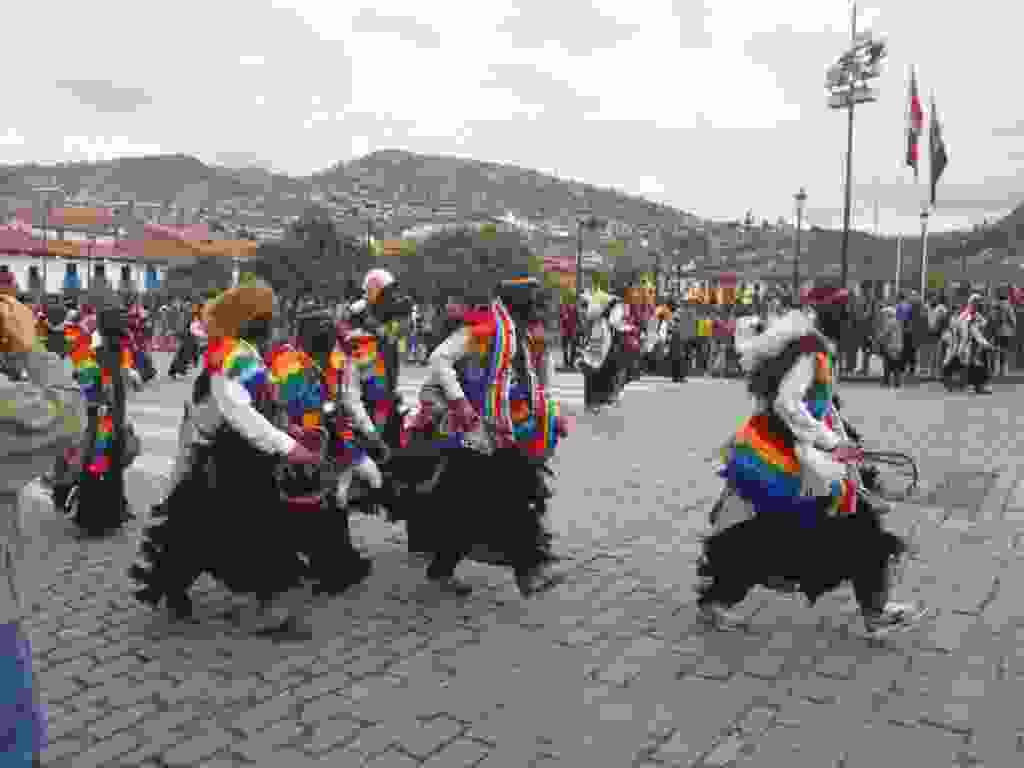
\includegraphics[width=\mywidth]{../wp-content/uploads/2015/05/P5174116-1024x768.jpg} \end{center}
~
\begin{center} 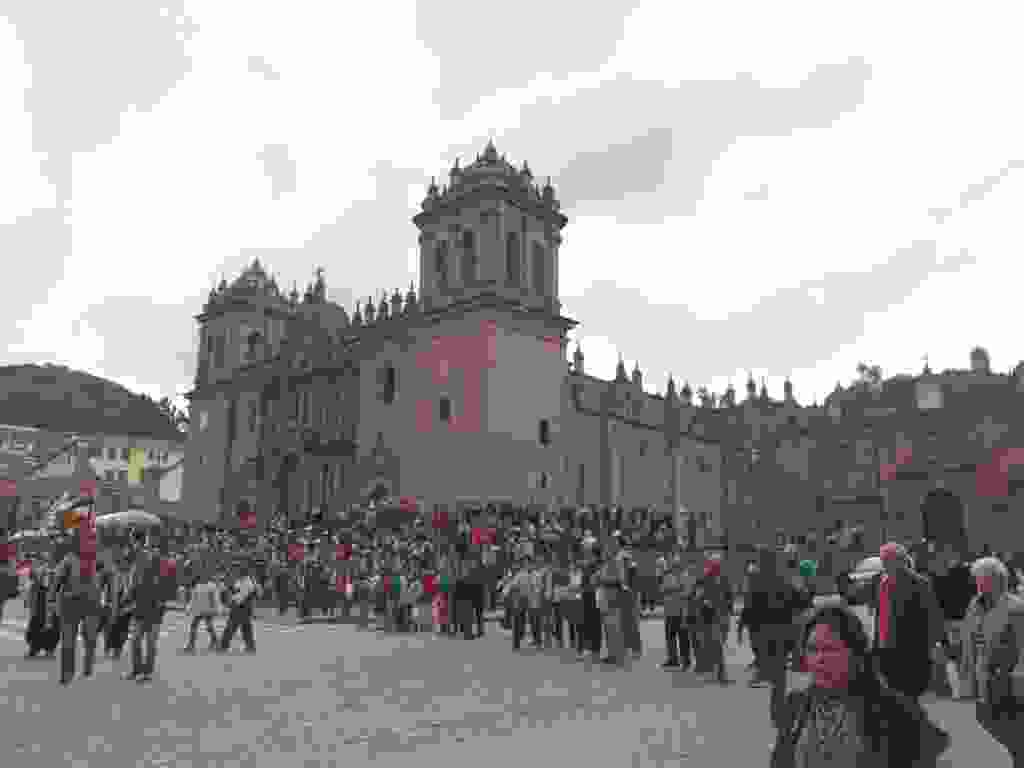
\includegraphics[width=\mywidth]{../wp-content/uploads/2015/05/P5174114-1024x768.jpg} \end{center}
\vspace{-\topsep}
\pagebreak
~
\begin{center} 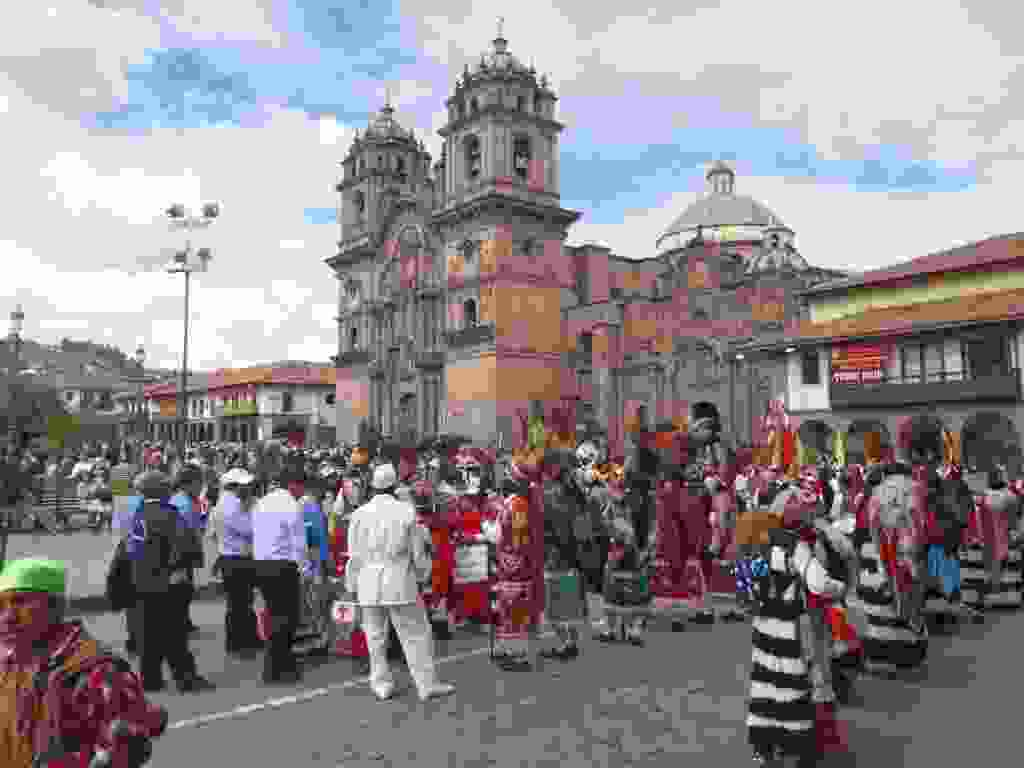
\includegraphics[width=\mywidth]{../wp-content/uploads/2015/05/P5174126-1024x768.jpg} \end{center}

Qorikancha : couvent construit par les espagnols sur un temple inca. 
\begin{center} 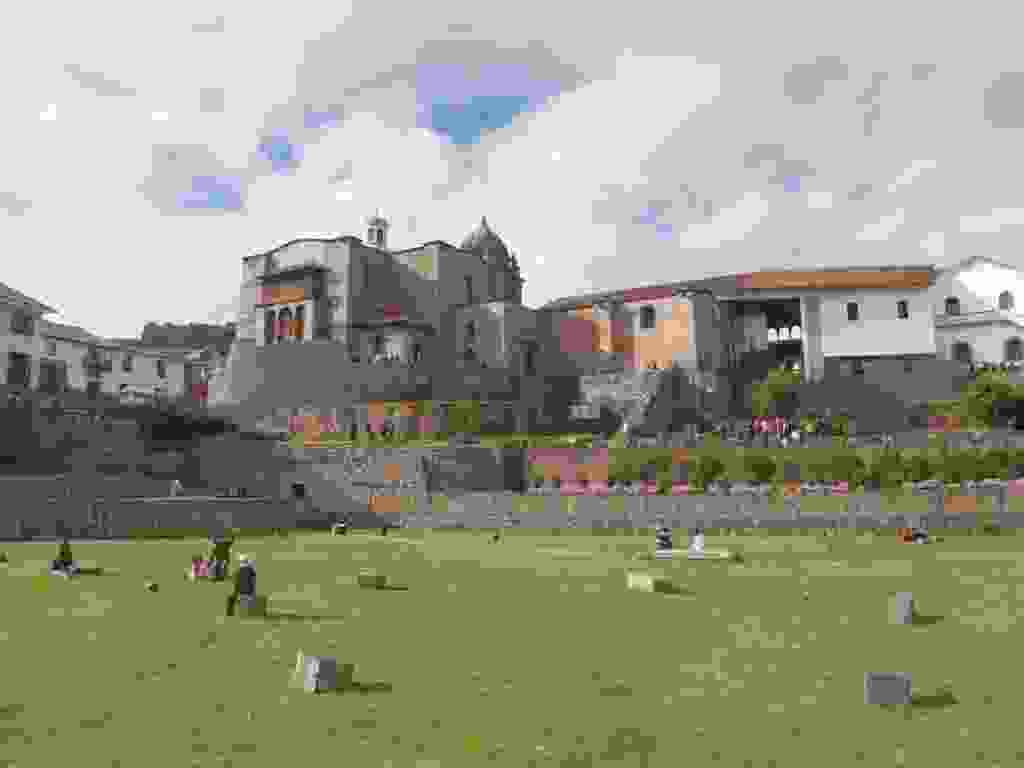
\includegraphics[width=\mywidth]{../wp-content/uploads/2015/05/P5174136-1024x768.jpg} \end{center}
\vspace{-\topsep}
\pagebreak
~\\
~\\
\vspace{-0.25mm}
\begin{center} 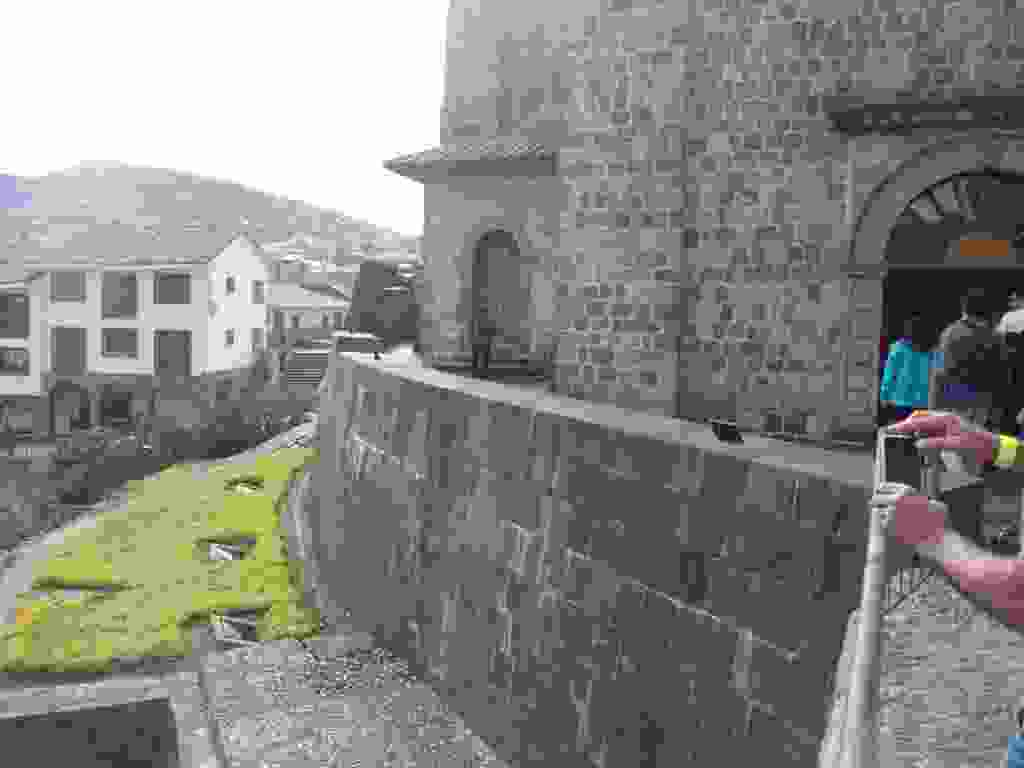
\includegraphics[width=\mywidth]{../wp-content/uploads/2015/05/P51741301-1024x768.jpg} \end{center}
\begin{center} 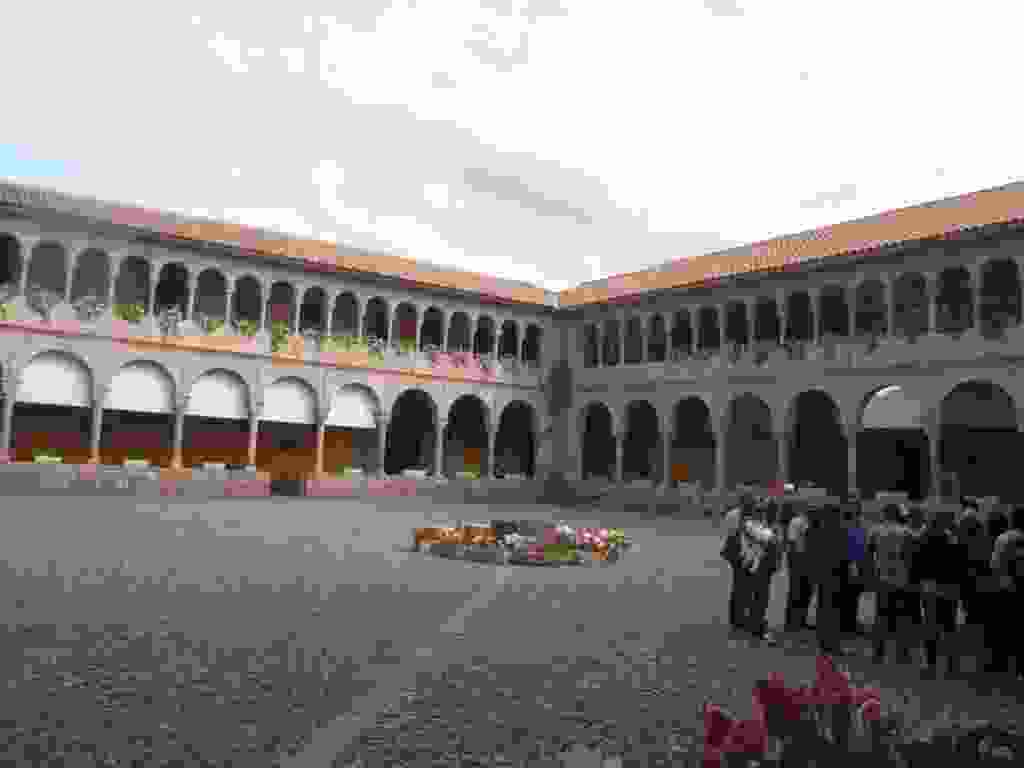
\includegraphics[width=\mywidth]{../wp-content/uploads/2015/05/P5174127-1024x768.jpg} \end{center}
\vspace{-\topsep}
\vspace{-2.5mm}
\pagebreak

Quatre sites archéologiques sont situés très proches de la ville : 
\begin{itemize}
\item Sacsayhuamán : forteresse inca construite avec des blocs de pierre énormes. 
\end{itemize}
\vspace{-\topsep}
\begin{center} 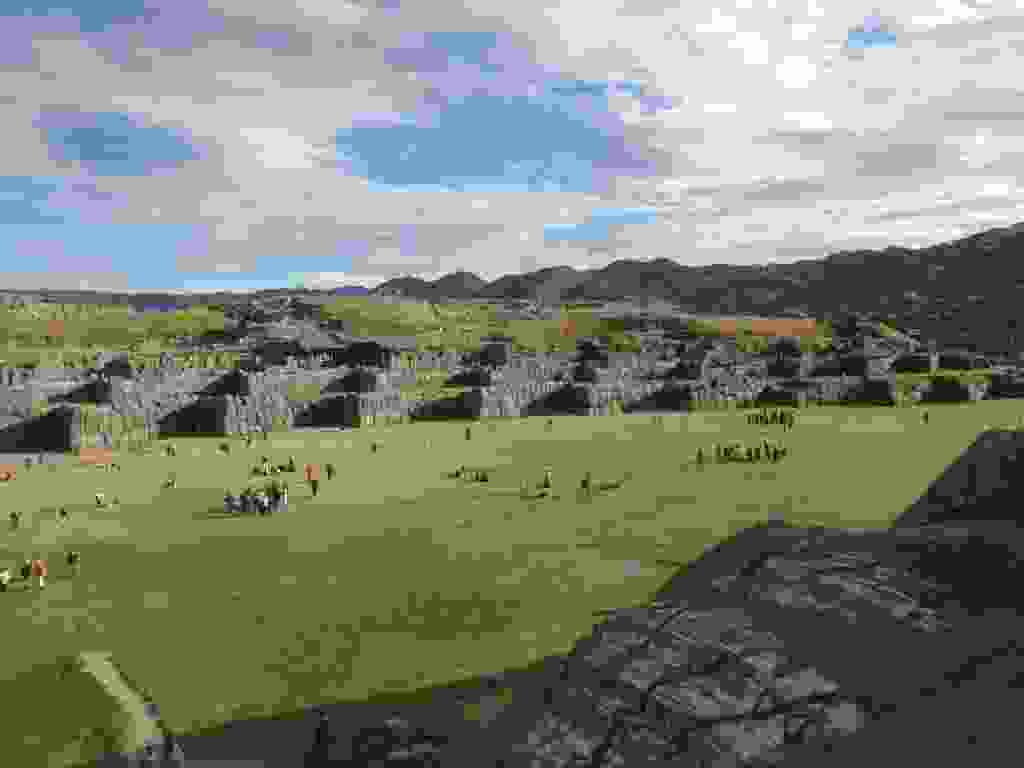
\includegraphics[width=\mywidth]{../wp-content/uploads/2015/05/P5174147-1024x768.jpg} \end{center}
\begin{center} 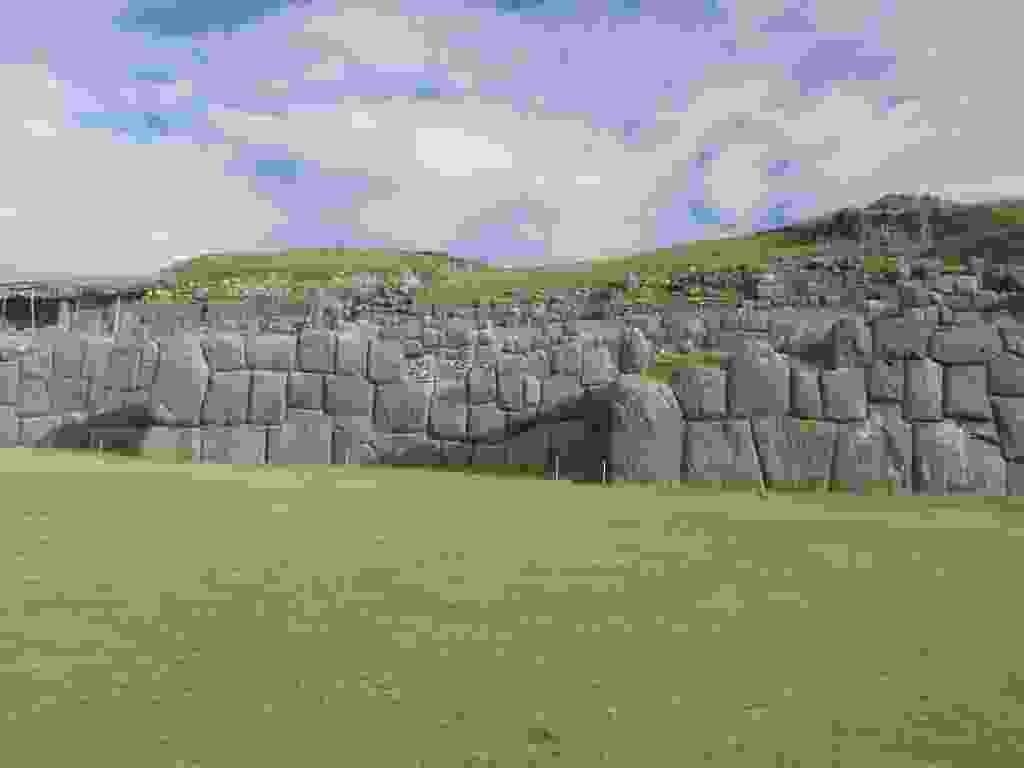
\includegraphics[width=\mywidth]{../wp-content/uploads/2015/05/P5174139-1024x768.jpg} \end{center}
\vspace{-\topsep}
\vspace{-2.75mm}
\pagebreak
\begin{itemize}
\item Qenko : ancien lieu de culte.
\end{itemize}
\vspace{2mm}
\begin{center} 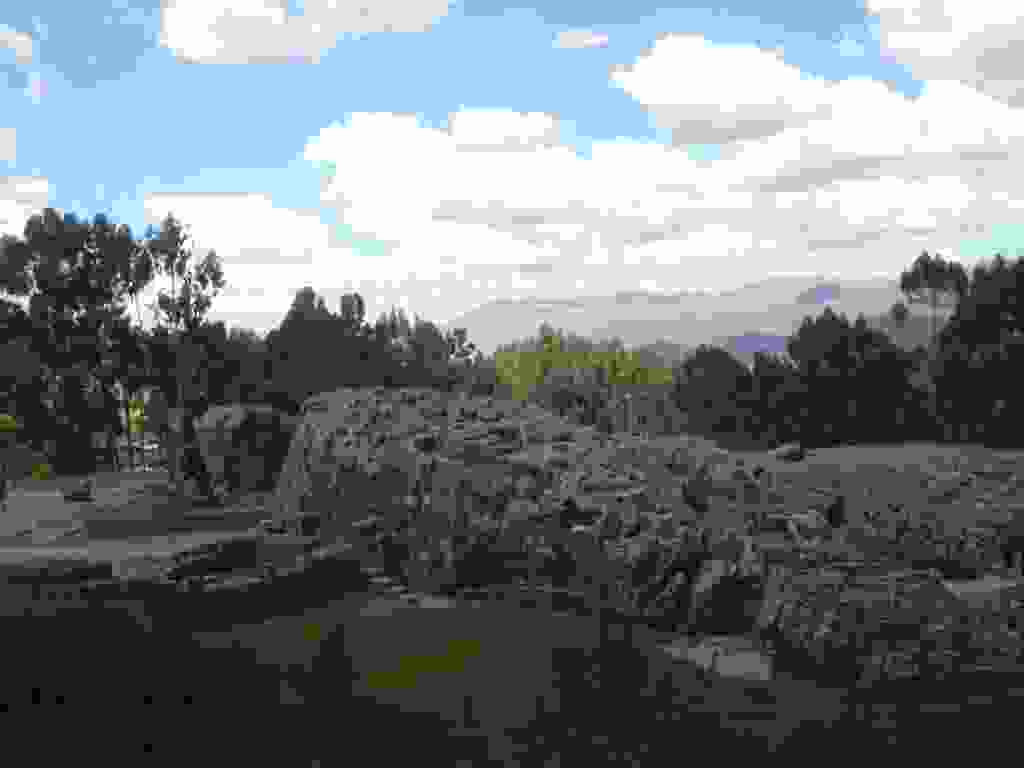
\includegraphics[width=\mywidth]{../wp-content/uploads/2015/05/P5224334-1024x768.jpg} \end{center}
\begin{itemize}
\item Pukapukara : poste militaire inca. 
\end{itemize}
\begin{center} 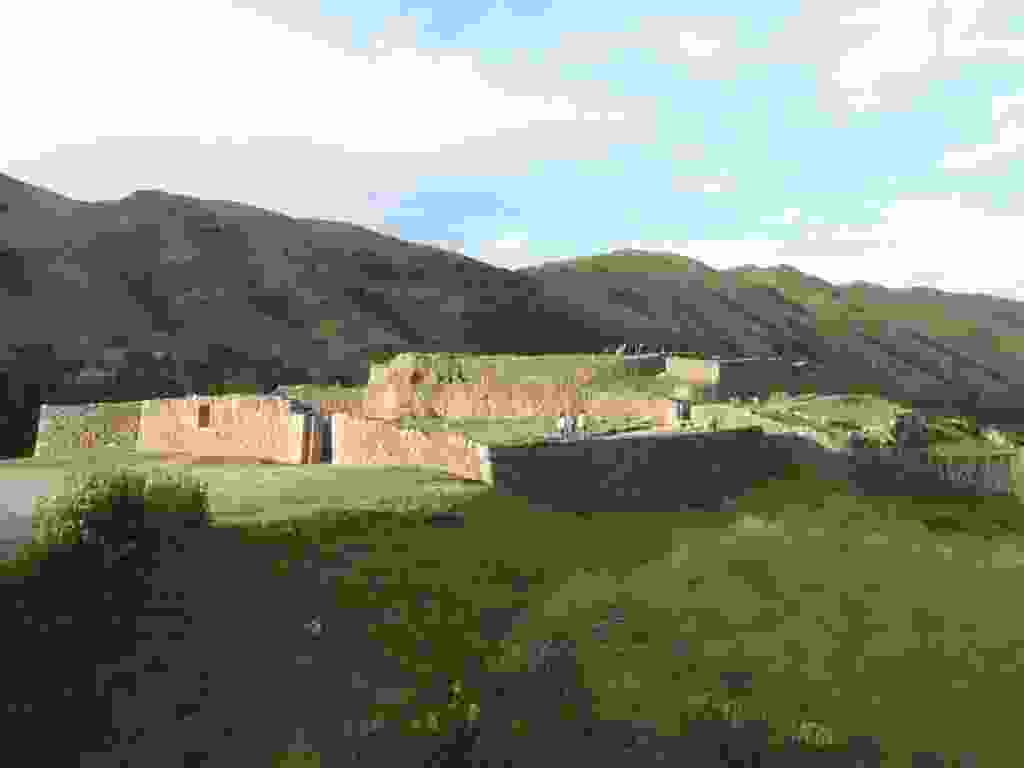
\includegraphics[width=\mywidth]{../wp-content/uploads/2015/05/P5174150-1024x768.jpg} \end{center}
\vspace{-\topsep}
\vspace{-1.5mm}
\pagebreak
\begin{itemize}
\item Tambomachay : point de passage et de cérémonie sur le chemin de l'inca. 
\end{itemize}
\begin{center} 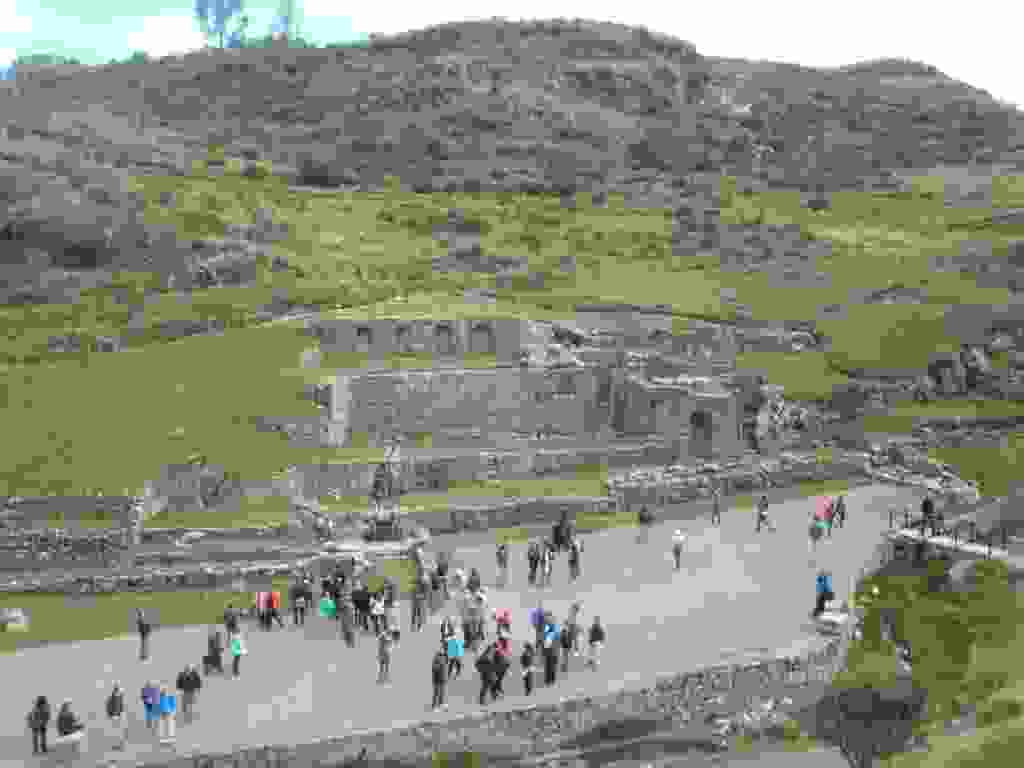
\includegraphics[width=\mywidth]{../wp-content/uploads/2015/05/P5184153-1024x768.jpg} \end{center}

Un spectacle de musique et danse traditionnelle est joué tous les soirs à Cusco. 
\begin{center} 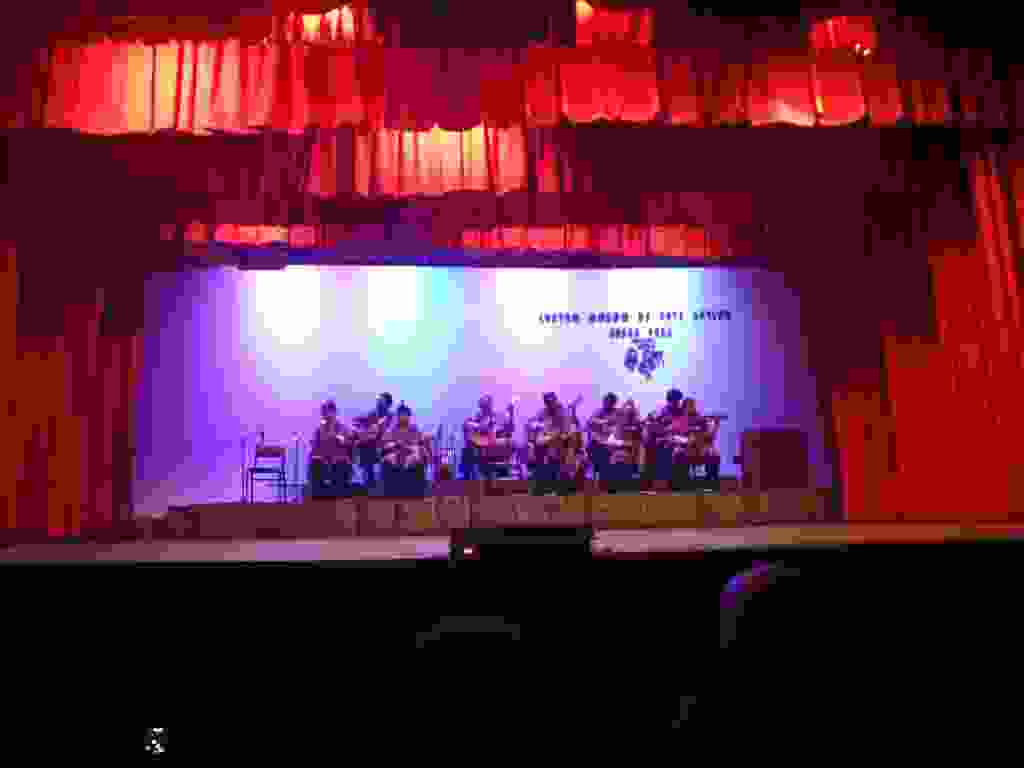
\includegraphics[width=\mywidth]{../wp-content/uploads/2015/05/P5194167-1024x768.jpg} \end{center}
\begin{center} 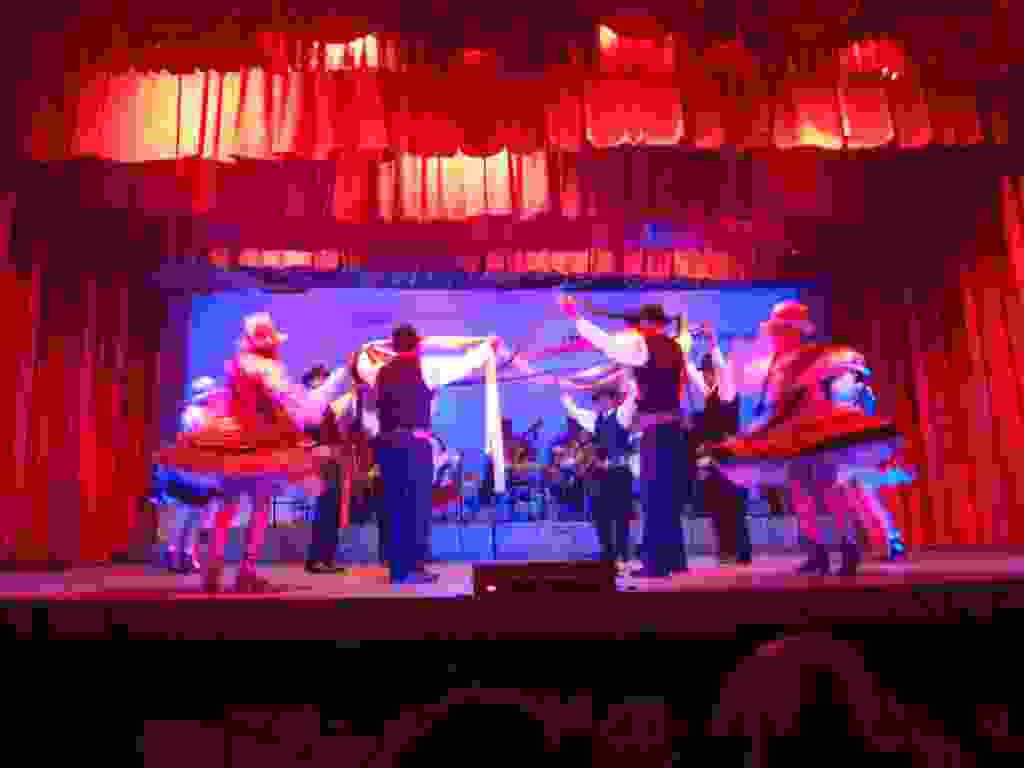
\includegraphics[width=\mywidth]{../wp-content/uploads/2015/05/P5194170-1024x768.jpg} \end{center}

Je suis parti 3 jours de Cusco pour faire le tour de la vallée sacrée des incas dont la particularité est d'être alignée avec la voie lactée. 
\begin{center} 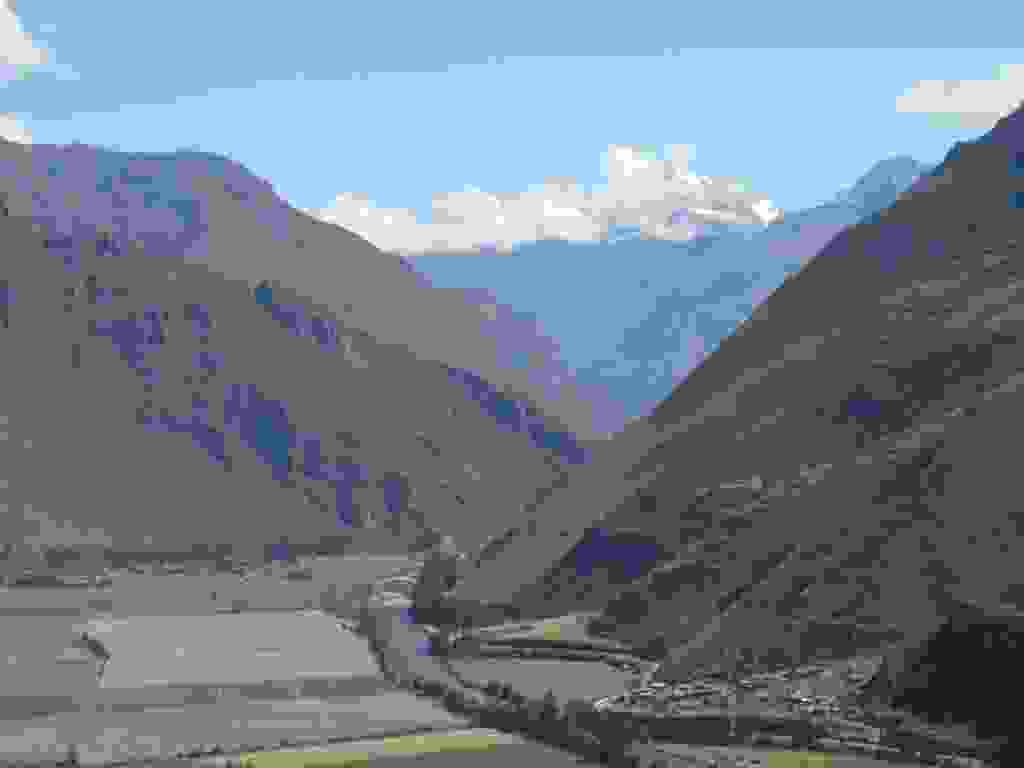
\includegraphics[width=\mywidth]{../wp-content/uploads/2015/05/P5224311-1024x768.jpg} \end{center}
\begin{center} 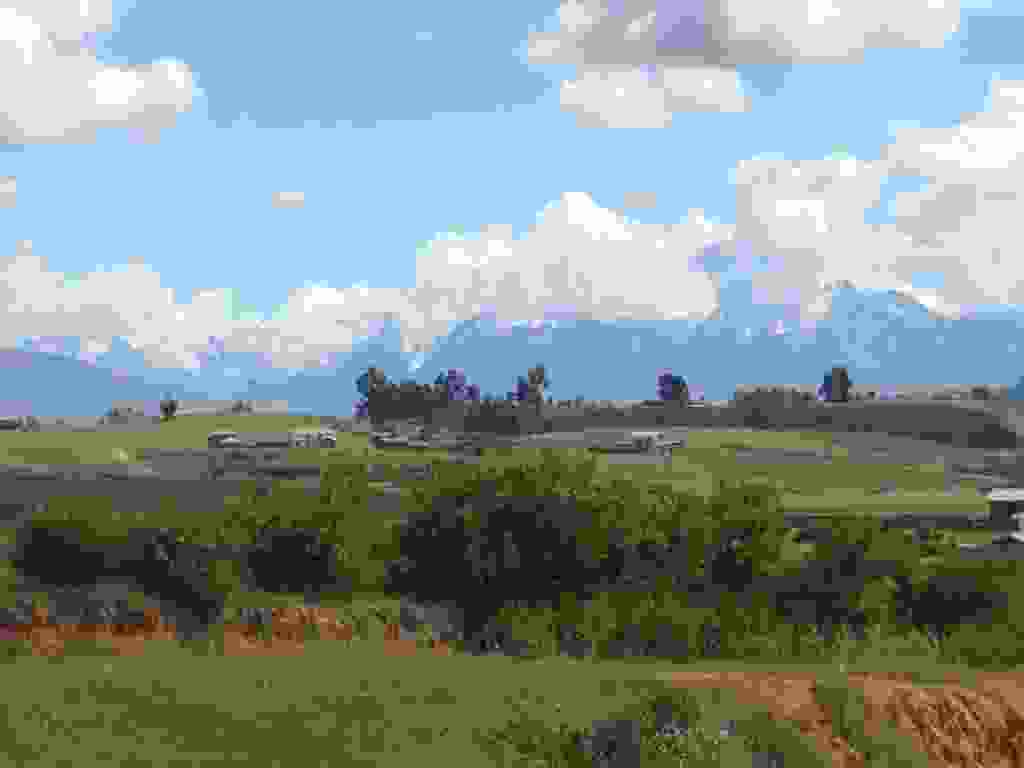
\includegraphics[width=\mywidth]{../wp-content/uploads/2015/05/P5204185-1024x768.jpg} \end{center}
\begin{center} 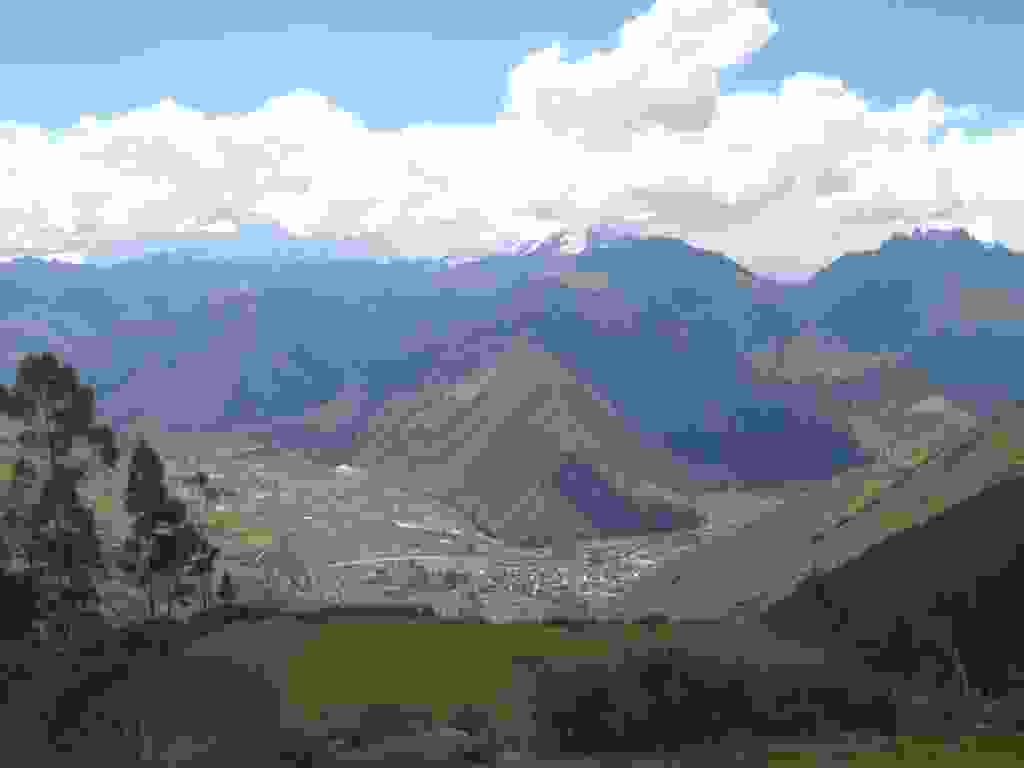
\includegraphics[width=\mywidth]{../wp-content/uploads/2015/05/P5204203-1024x768.jpg} \end{center}
\begin{center} 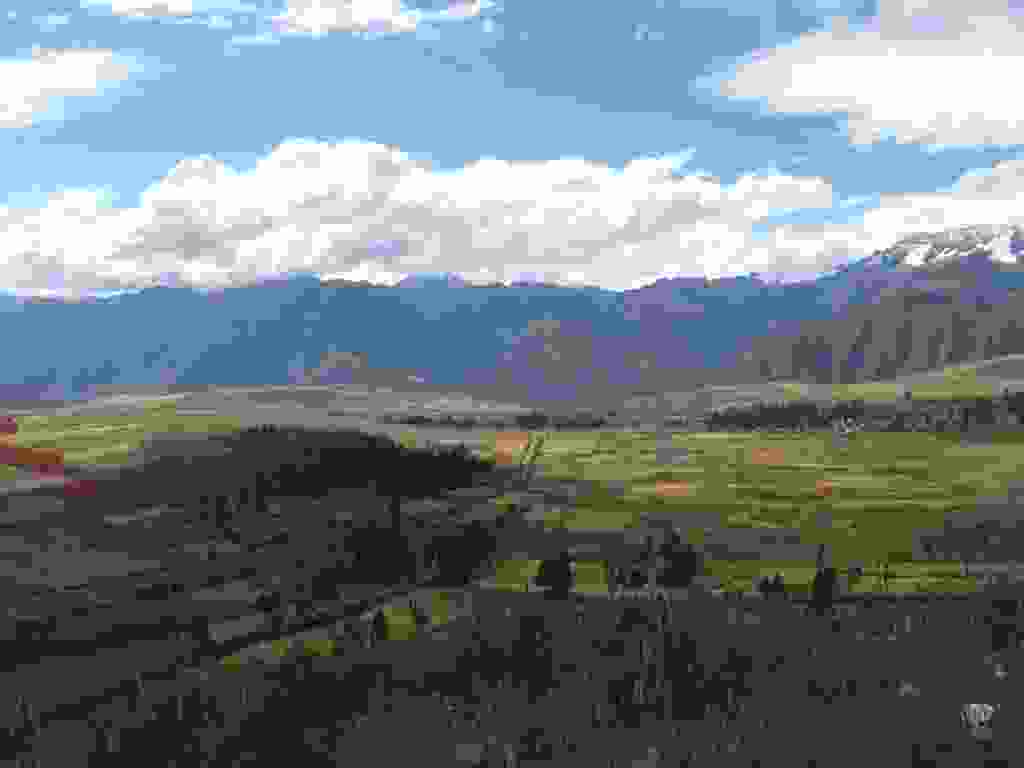
\includegraphics[width=\mywidth]{../wp-content/uploads/2015/05/P5204212-1024x768.jpg} \end{center}

En route, le site de Chinchero. 
\begin{center} 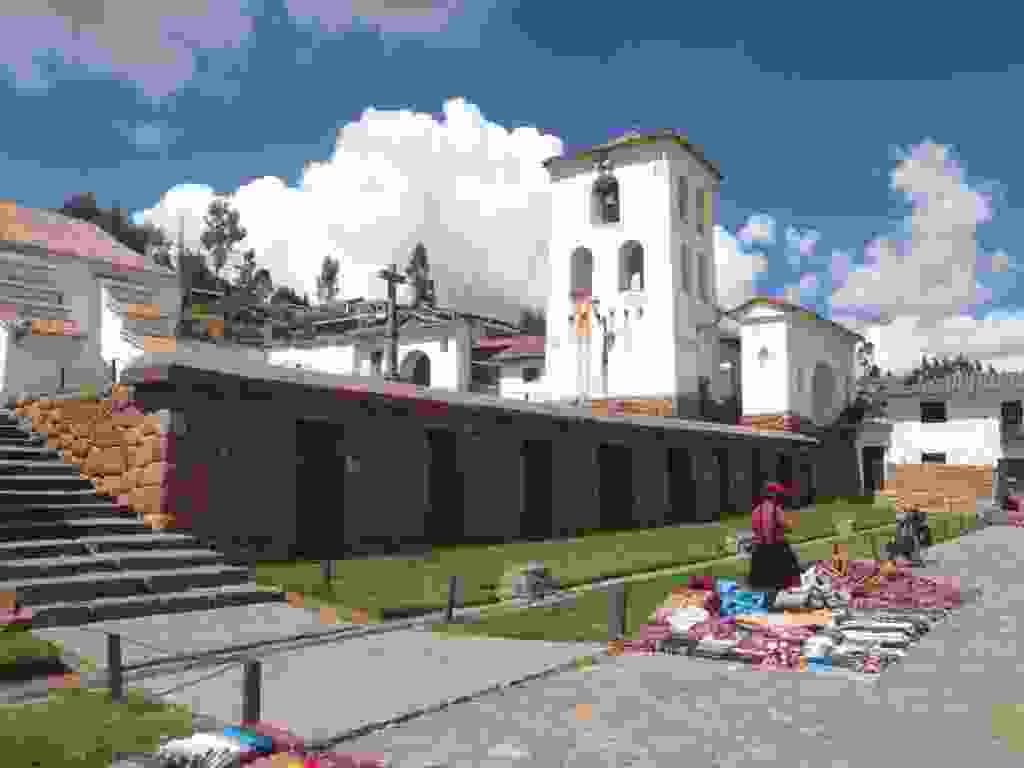
\includegraphics[width=\mywidth]{../wp-content/uploads/2015/05/P5204187-1024x768.jpg} \end{center}
\begin{center} 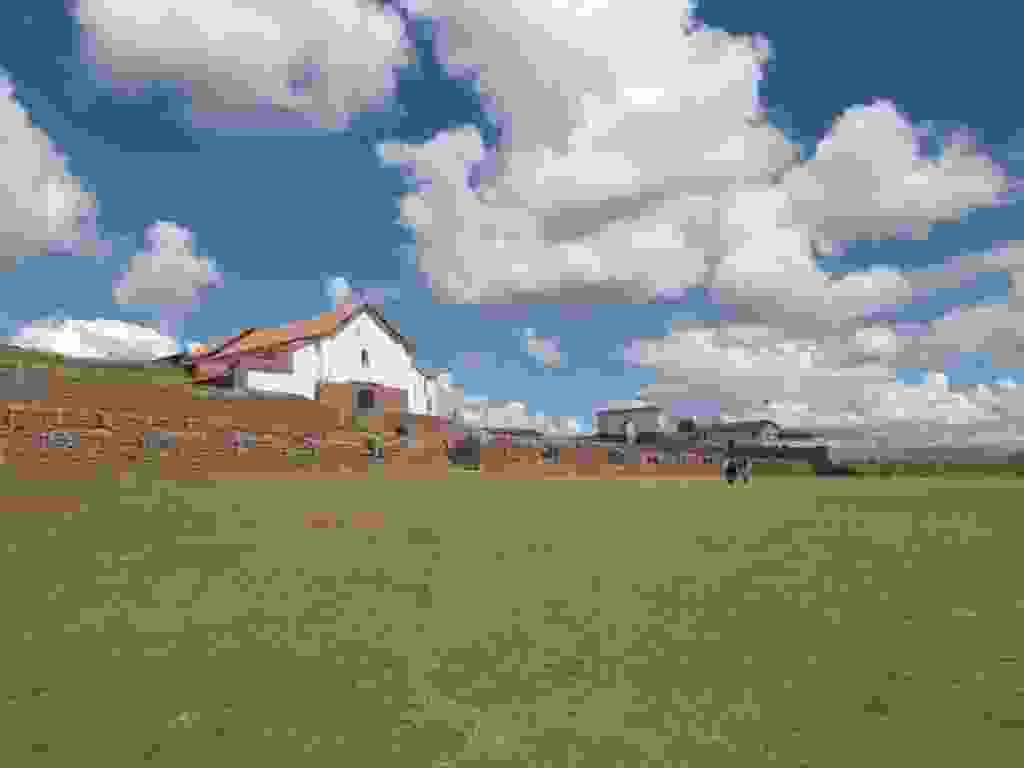
\includegraphics[width=\mywidth]{../wp-content/uploads/2015/05/P5204191-1024x768.jpg} \end{center}
\begin{center} 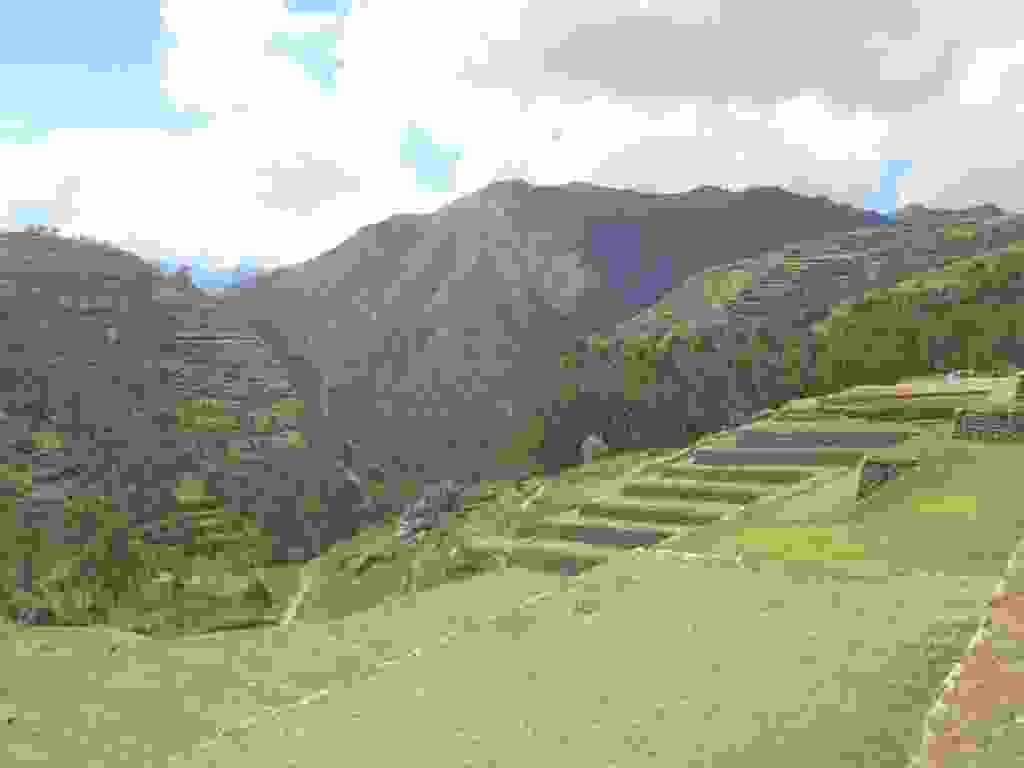
\includegraphics[width=\mywidth]{../wp-content/uploads/2015/05/P5204194-1024x768.jpg} \end{center}
\begin{center} 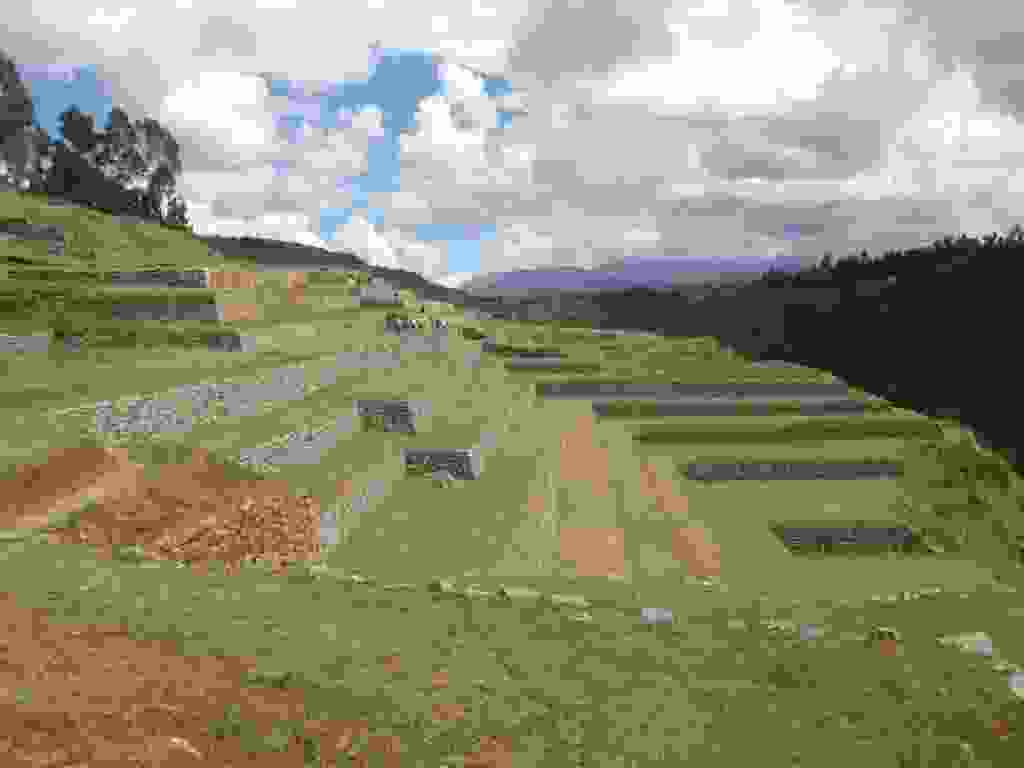
\includegraphics[width=\mywidth]{../wp-content/uploads/2015/05/P5204198-1024x768.jpg} \end{center}

Je visite Moray, un lieu d'expérimentations agricoles pour les incas permettant de reproduire différents microclimats. 
\begin{center} 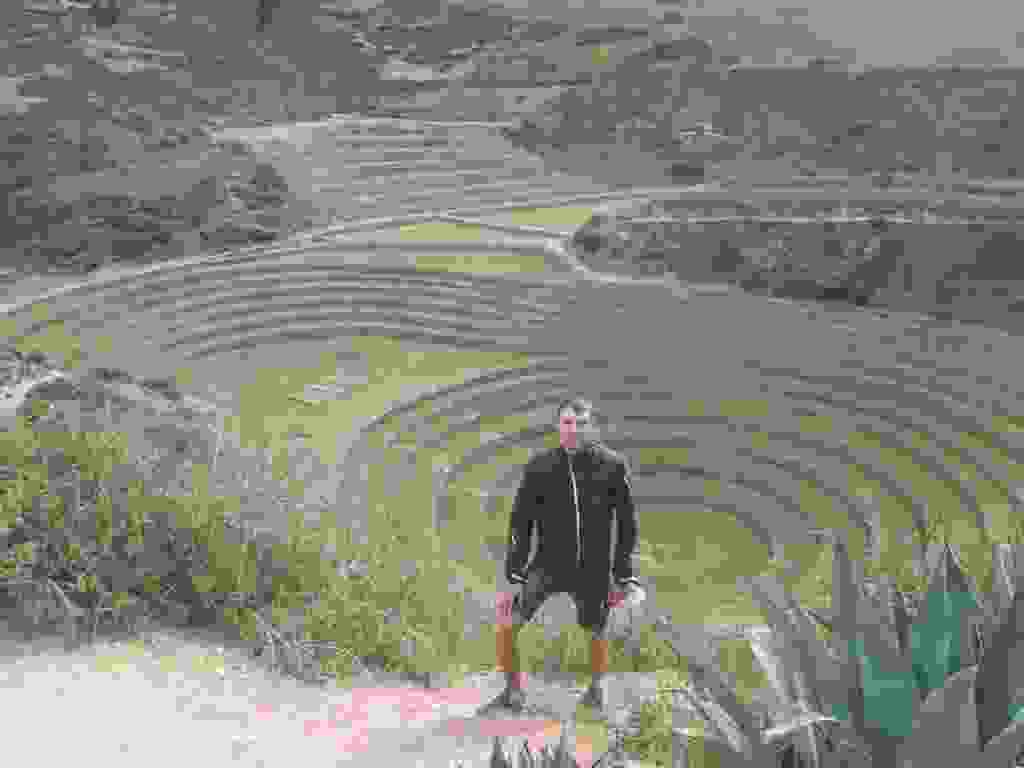
\includegraphics[width=\mywidth]{../wp-content/uploads/2015/05/P5204231-1024x768.jpg} \end{center}
\begin{center} 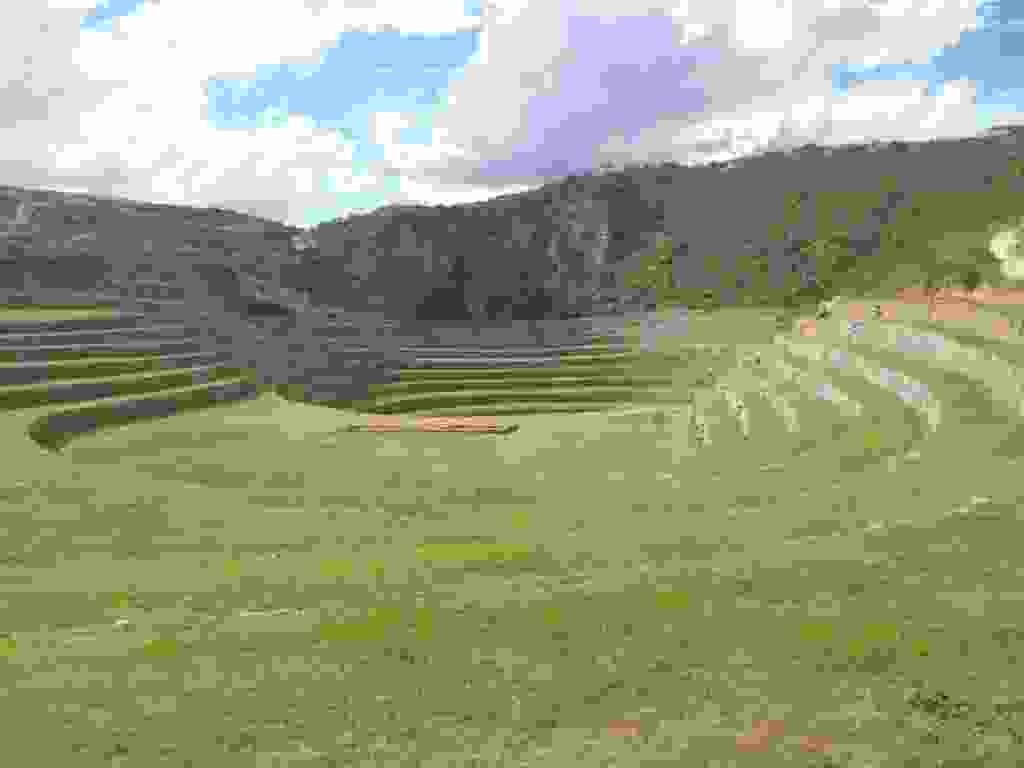
\includegraphics[width=\mywidth]{../wp-content/uploads/2015/05/P5204216-1024x768.jpg} \end{center}
\begin{center} 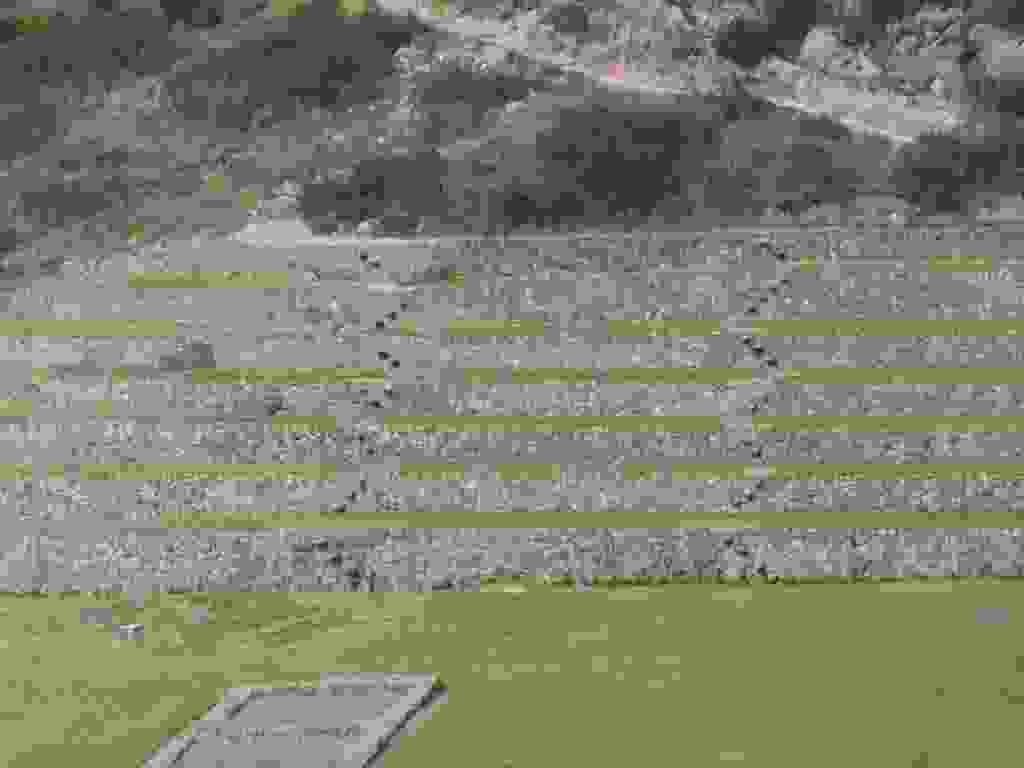
\includegraphics[width=\mywidth]{../wp-content/uploads/2015/05/P5204217-1024x768.jpg} \end{center}
\begin{center} 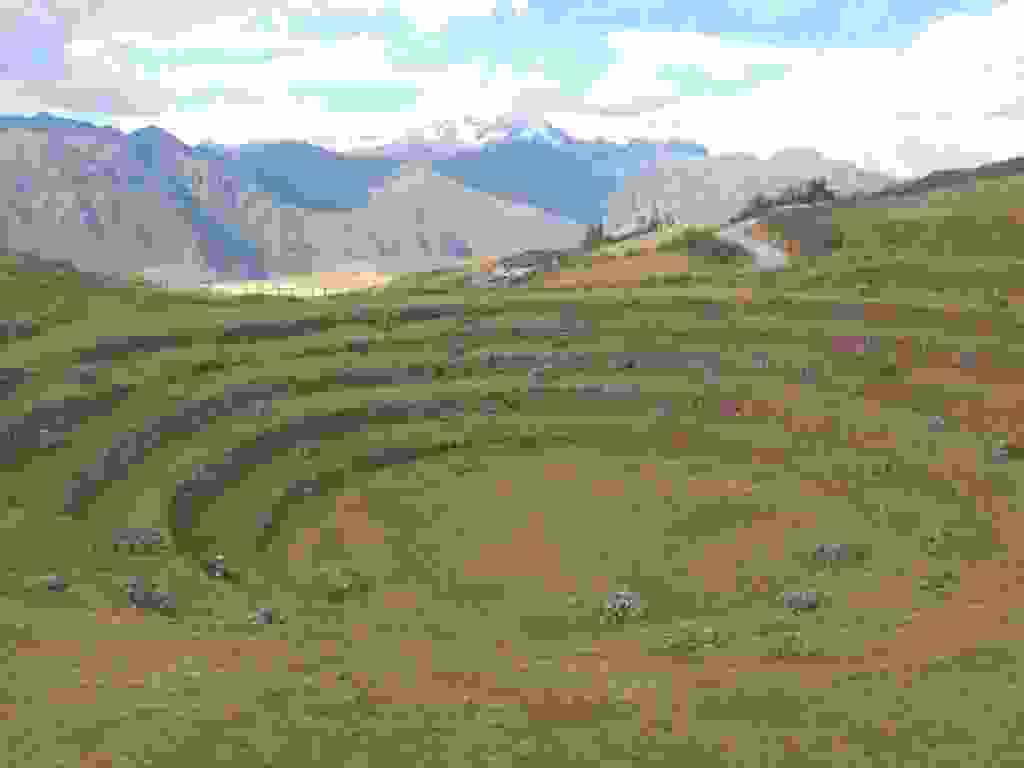
\includegraphics[width=\mywidth]{../wp-content/uploads/2015/05/P5204223-1024x768.jpg} \end{center}

Puis magnifique descente vers les Salineras de Maras datant de l'époque pré-inca et encore exploitées aujourd'hui. 
\begin{center} 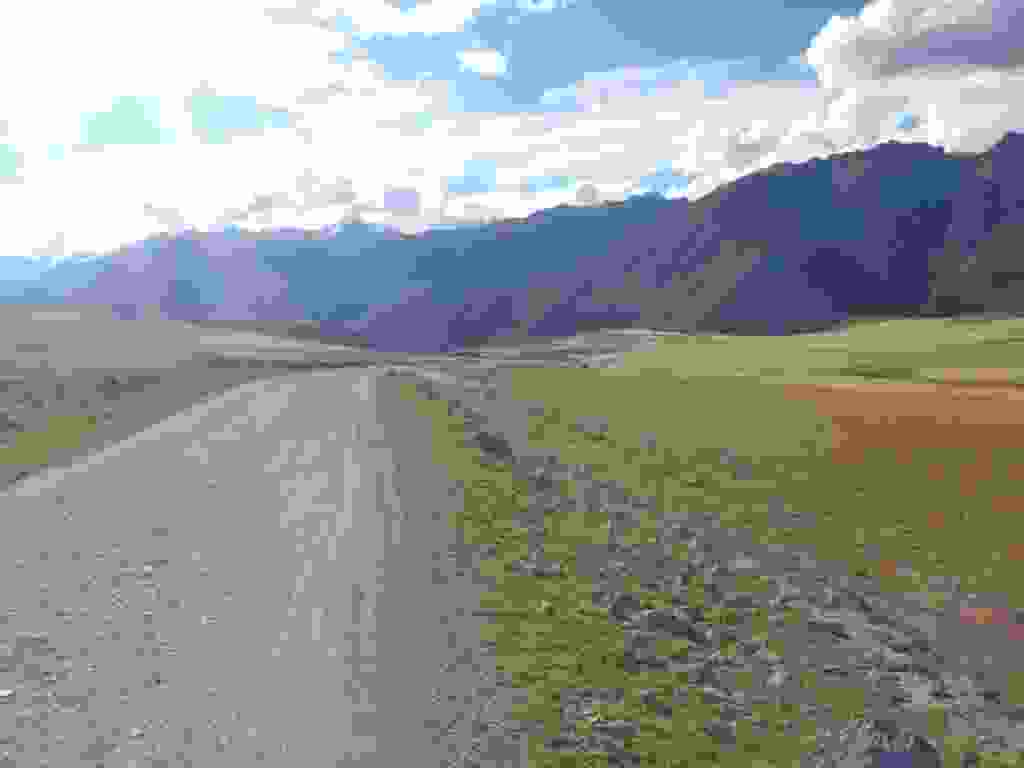
\includegraphics[width=\mywidth]{../wp-content/uploads/2015/05/P5204235-1024x768.jpg} \end{center}
\begin{center} 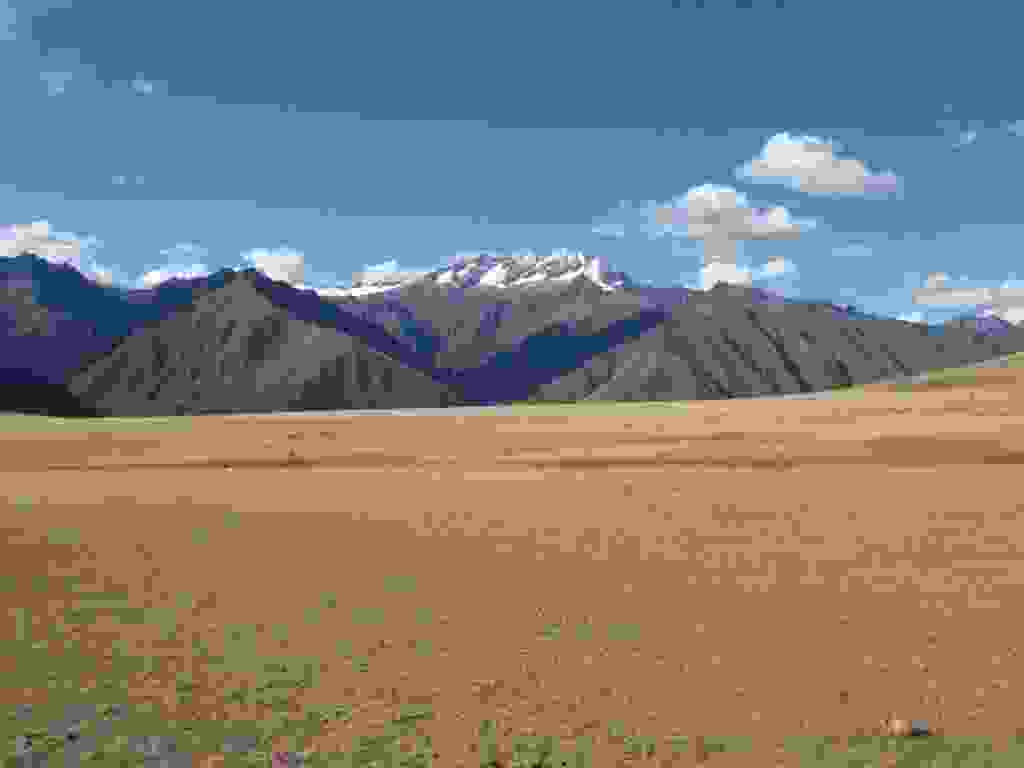
\includegraphics[width=\mywidth]{../wp-content/uploads/2015/05/P5204236-1024x768.jpg} \end{center}
\vfill
\begin{center} 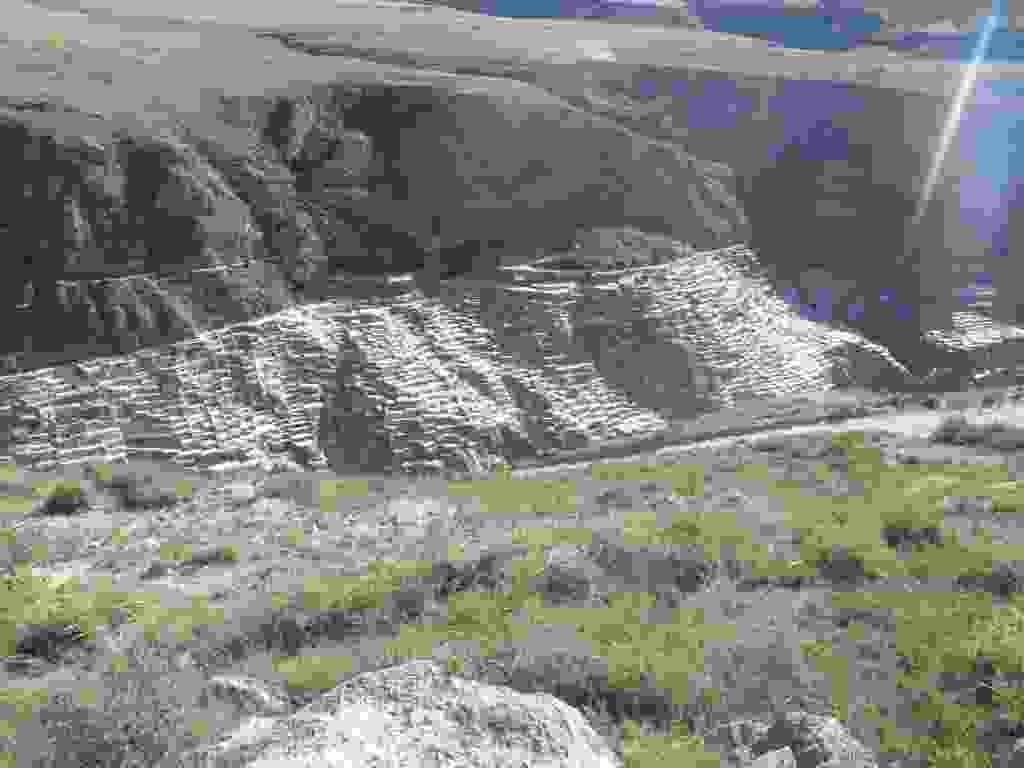
\includegraphics[width=\mywidth]{../wp-content/uploads/2015/05/P5204237-1024x768.jpg} \end{center}
\vspace{-\topsep}
\vspace{-0.75mm}
\pagebreak
~
\begin{center} 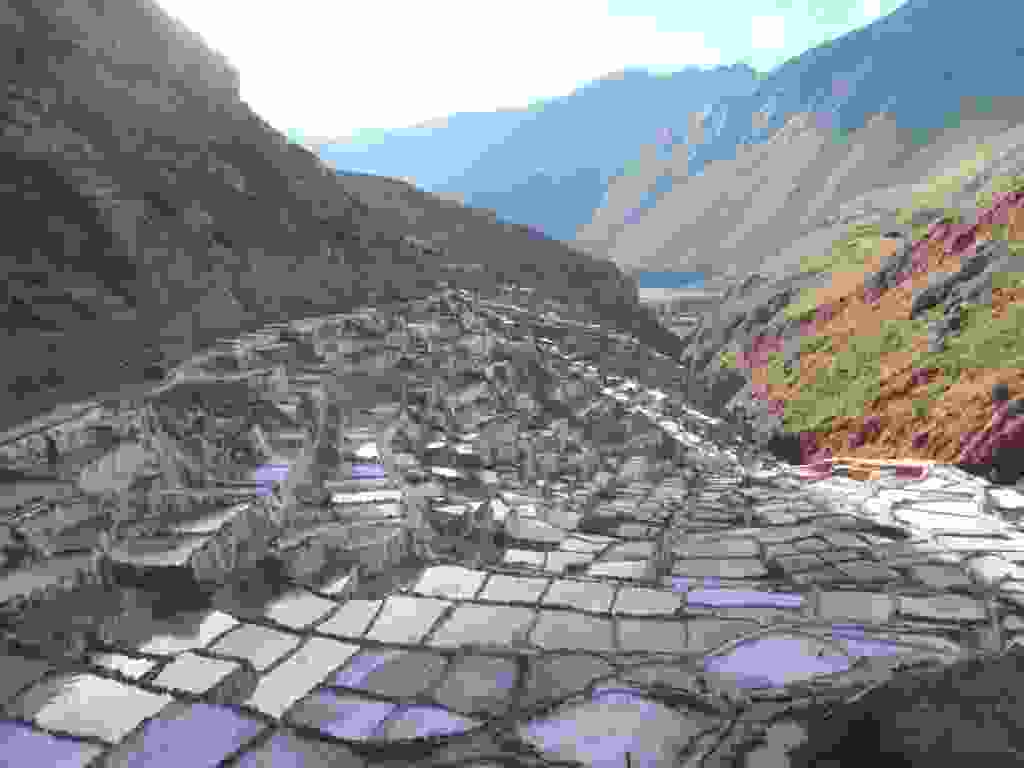
\includegraphics[width=\mywidth]{../wp-content/uploads/2015/05/P5204244-1024x768.jpg} \end{center}
\begin{center} 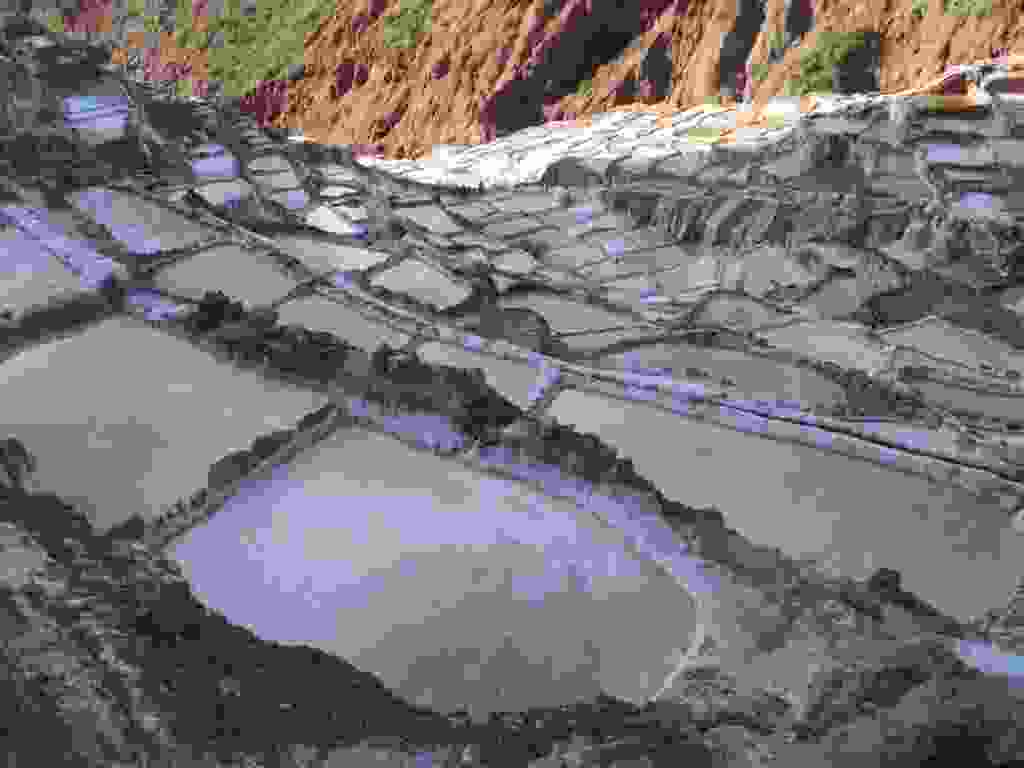
\includegraphics[width=\mywidth]{../wp-content/uploads/2015/05/P5204246-1024x768.jpg} \end{center}
\vspace{-\topsep}
\vspace{-3.25mm}
\pagebreak

Le lendemain, du plat pour traverser la vallée. 
\begin{center} 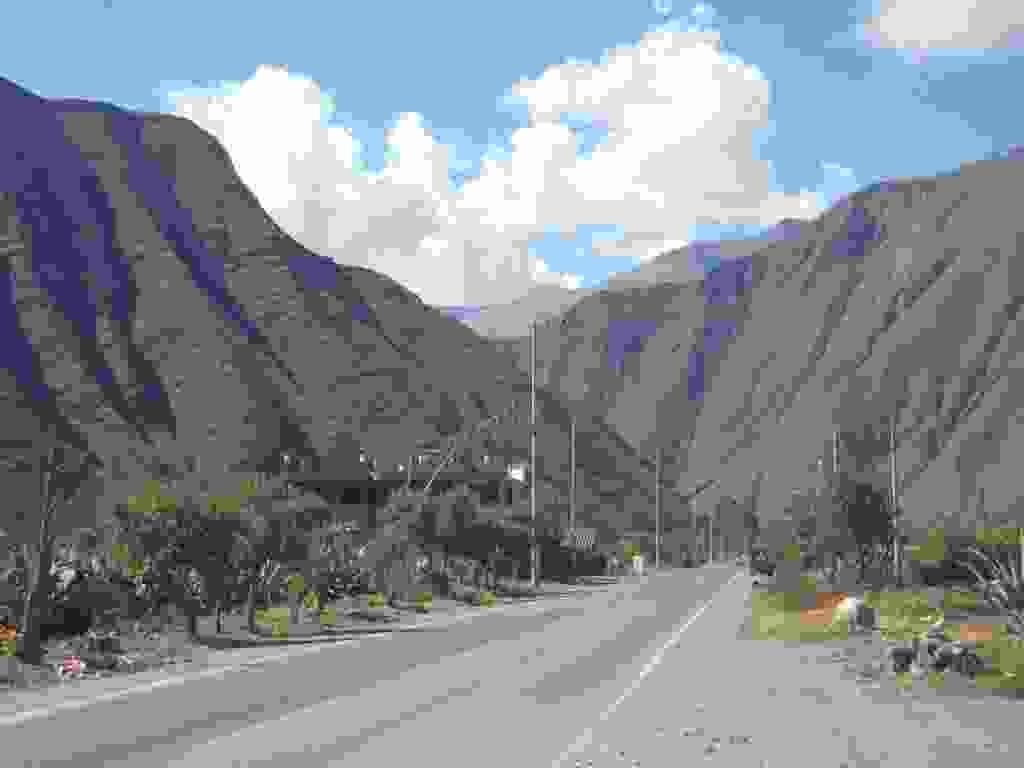
\includegraphics[width=\mywidth]{../wp-content/uploads/2015/05/P5214251-1024x768.jpg} \end{center}
\begin{center} 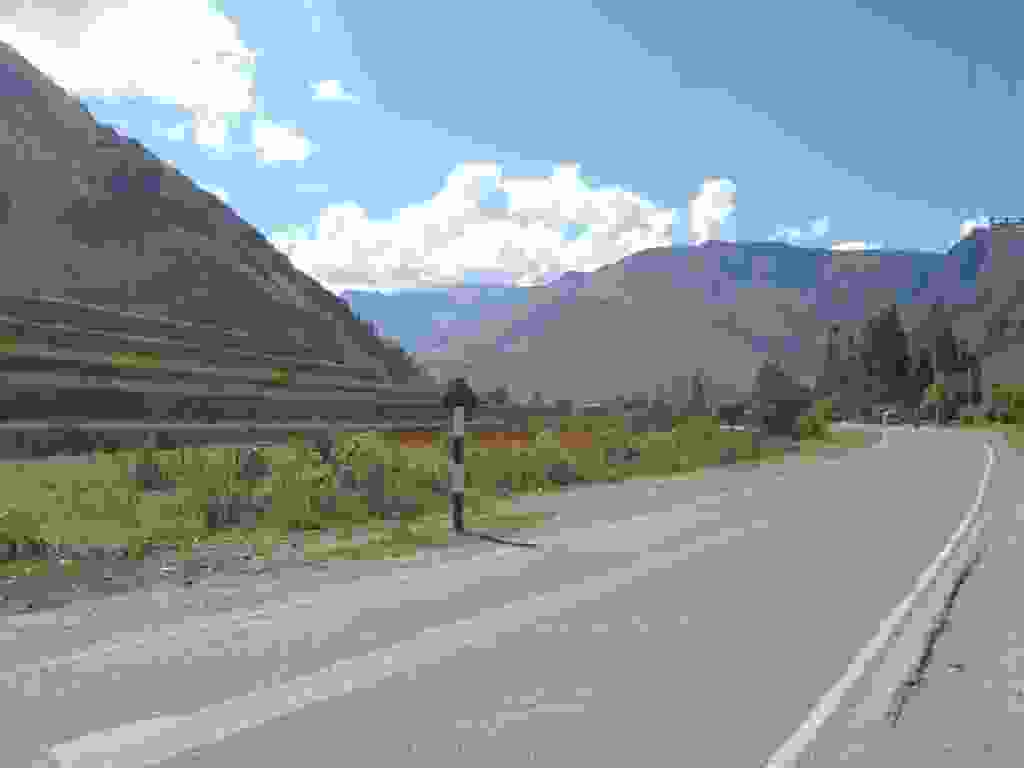
\includegraphics[width=\mywidth]{../wp-content/uploads/2015/05/P5214255-1024x768.jpg} \end{center}
\vspace{-\topsep}
\vspace{-3.25mm}
\pagebreak

Le jus de quinoa, bien pour prendre des forces. 
\begin{center} 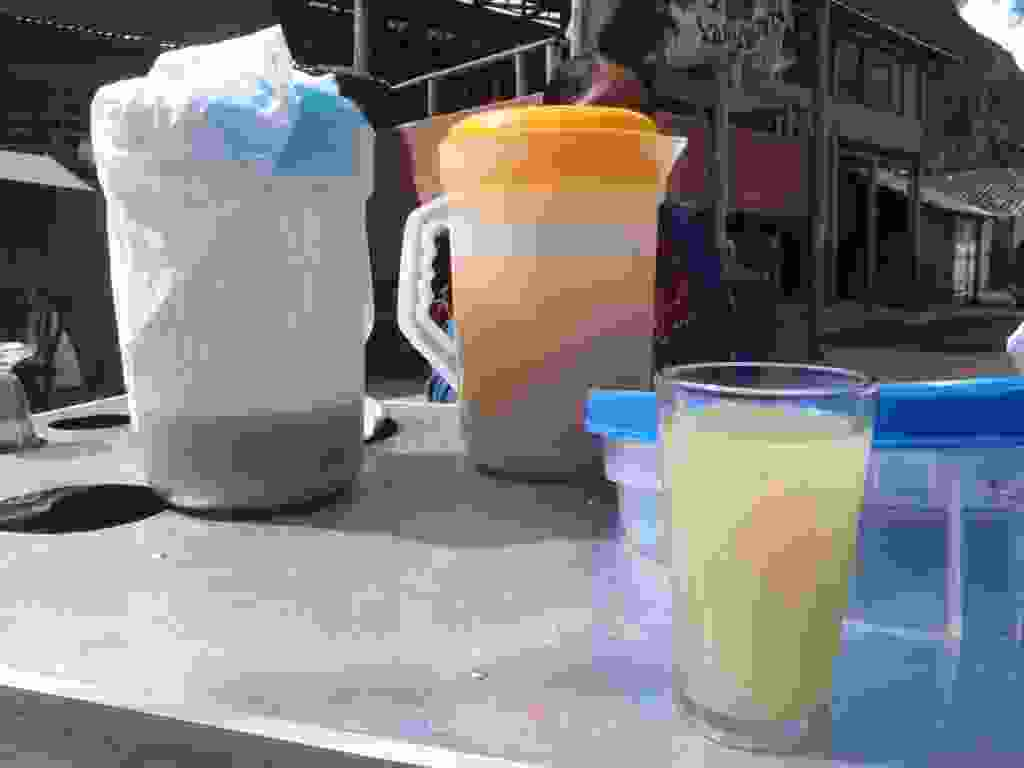
\includegraphics[width=\mywidth]{../wp-content/uploads/2015/05/P5214257-1024x768.jpg} \end{center}

Dans un village, des restaurants préparent la spécialité locale : le cochon d'Inde (je n'ai pas encore gouté !)
\begin{center} 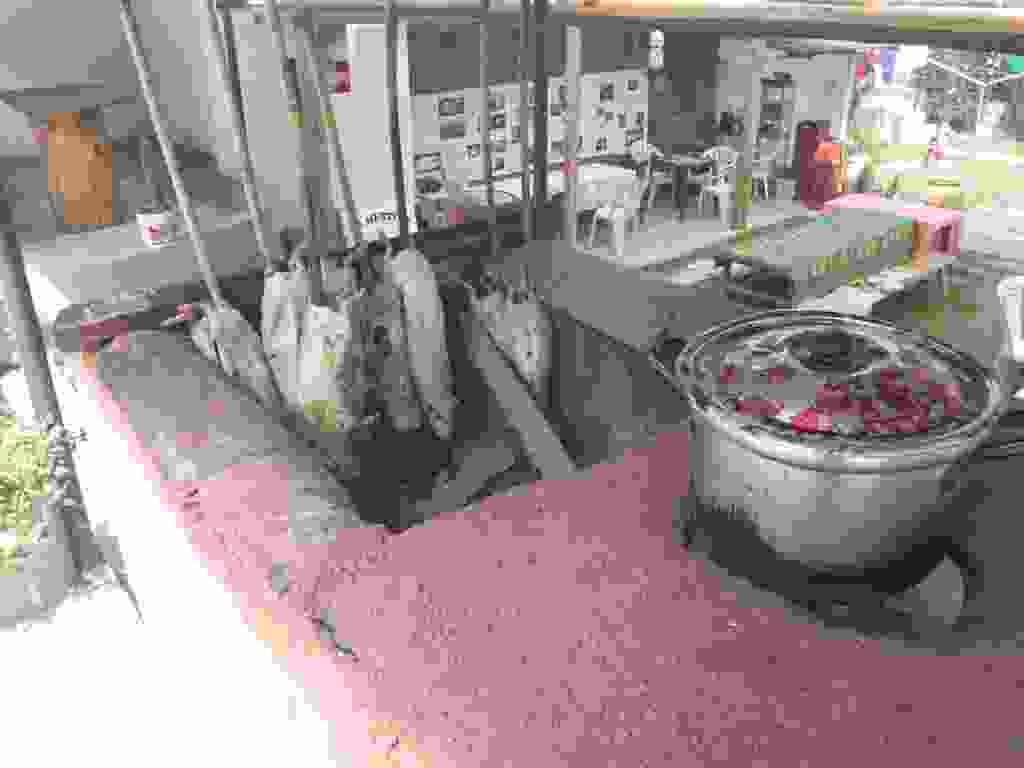
\includegraphics[width=\mywidth]{../wp-content/uploads/2015/05/P5214258-1024x768.jpg} \end{center}
\vspace{-\topsep}
\pagebreak

La vallée finit à Pisac, très beau site inca perché sur la montagne. 
\begin{center} 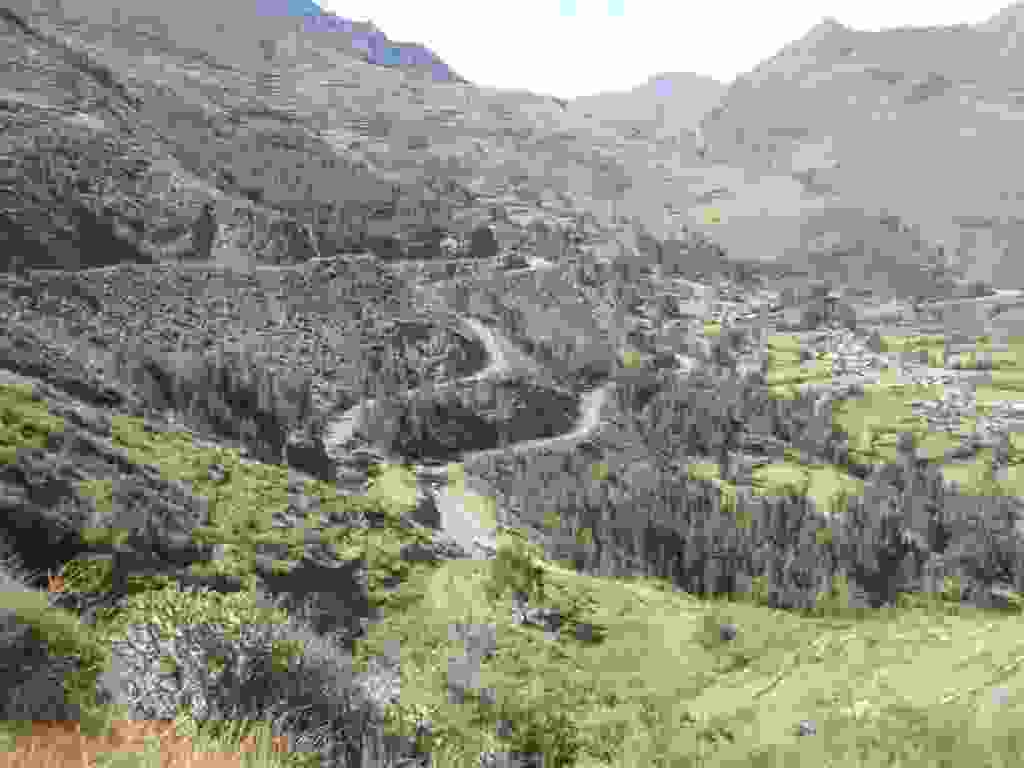
\includegraphics[width=\mywidth]{../wp-content/uploads/2015/05/P5214267-1024x768.jpg} \end{center}
~\\
\begin{center} 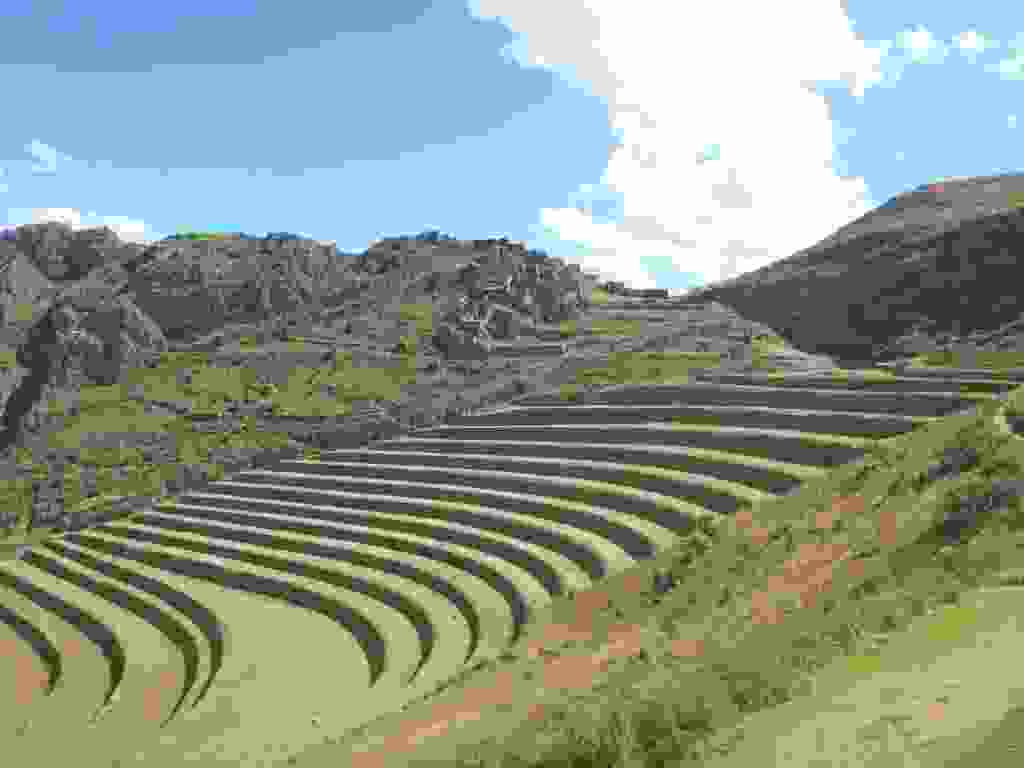
\includegraphics[width=\mywidth]{../wp-content/uploads/2015/05/P5214268-1024x768.jpg} \end{center}
\begin{center} 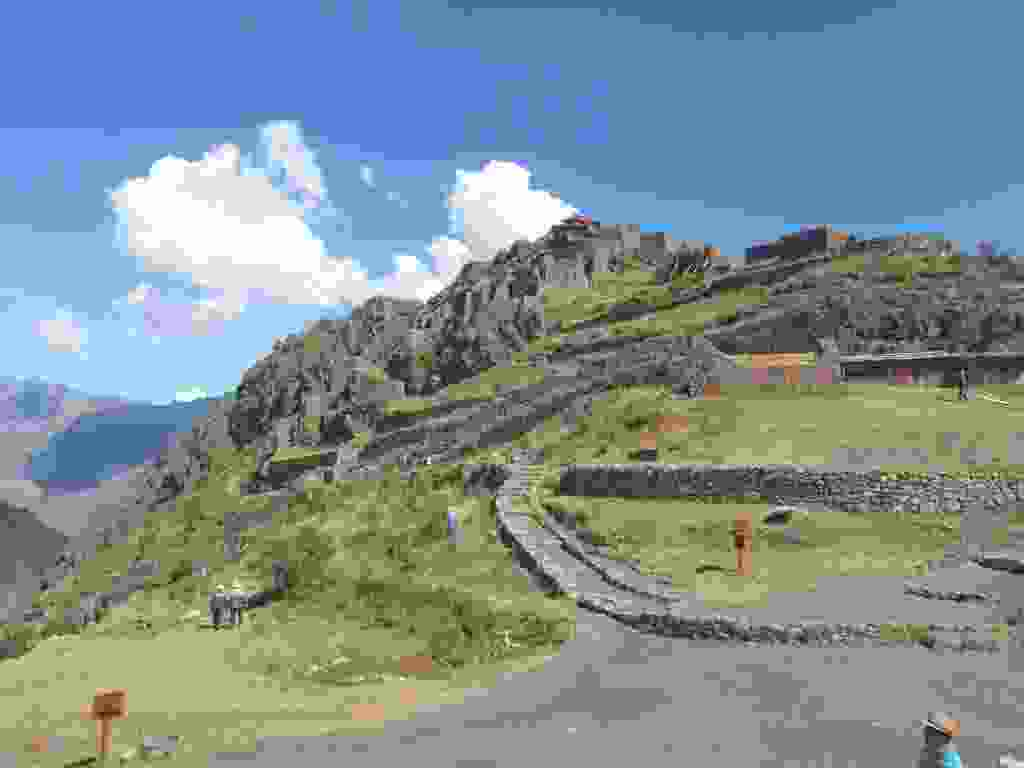
\includegraphics[width=\mywidth]{../wp-content/uploads/2015/05/P5214270-1024x768.jpg} \end{center}
\begin{center} 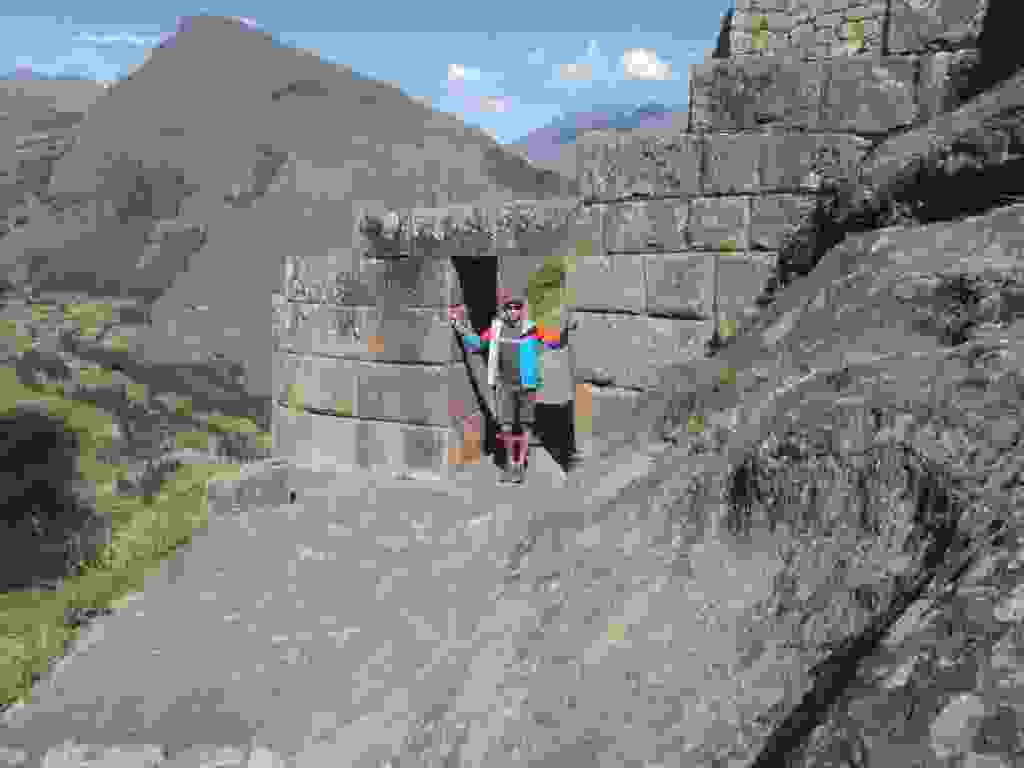
\includegraphics[width=\mywidth]{../wp-content/uploads/2015/05/P5214274-1024x768.jpg} \end{center}
\begin{center} 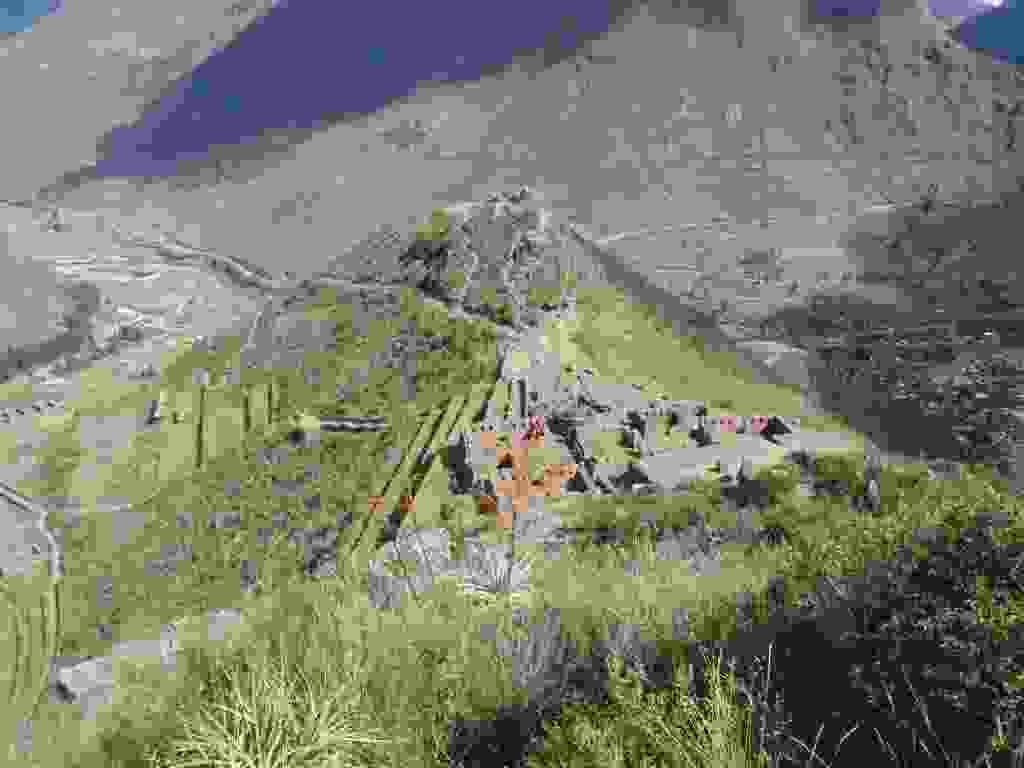
\includegraphics[width=\mywidth]{../wp-content/uploads/2015/05/P5214283-1024x768.jpg} \end{center}
\begin{center} 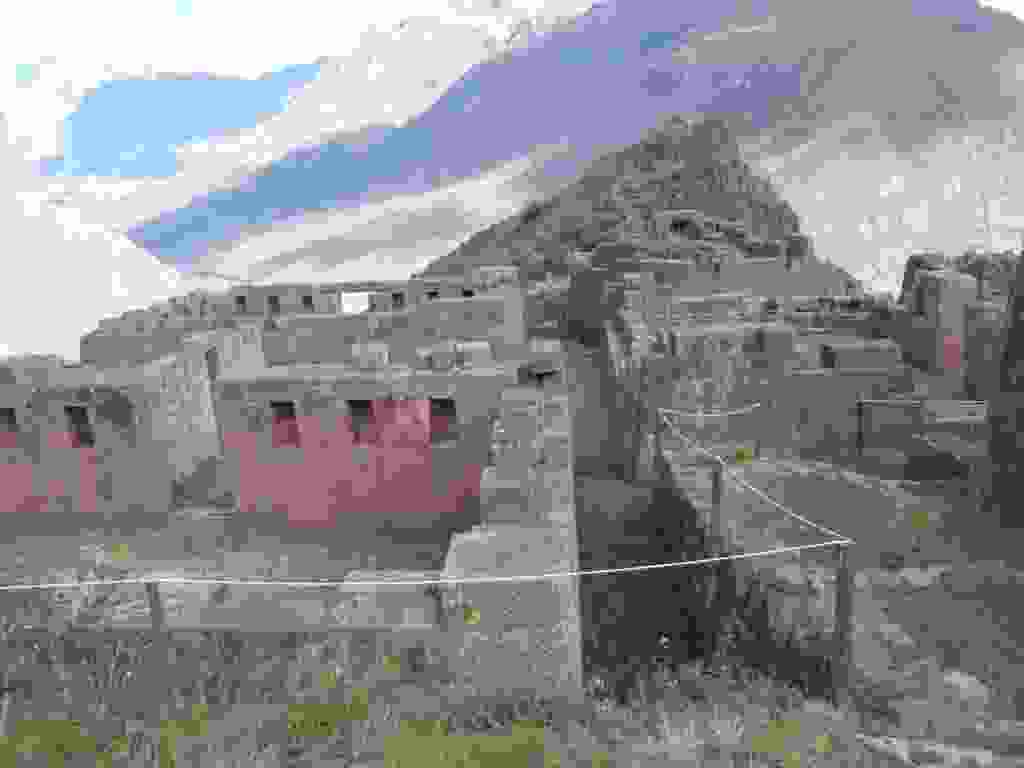
\includegraphics[width=\mywidth]{../wp-content/uploads/2015/05/P5214286-1024x768.jpg} \end{center}
\begin{center} 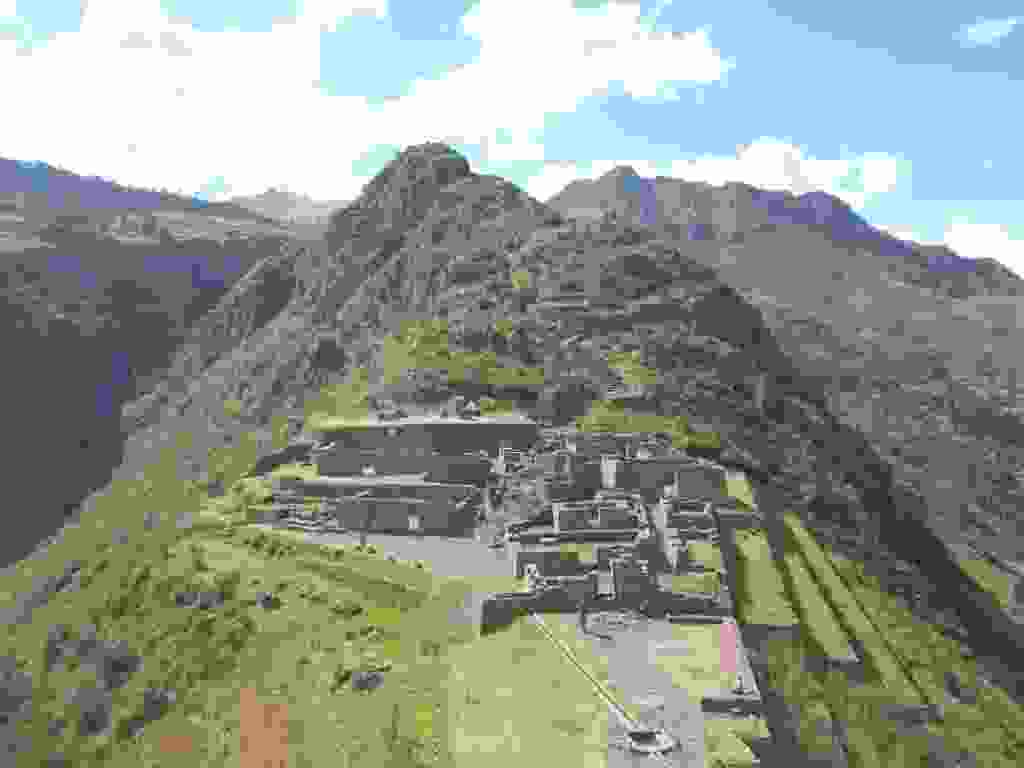
\includegraphics[width=\mywidth]{../wp-content/uploads/2015/05/P5214289-1024x768.jpg} \end{center}

Retour à Cusco avec une bonne montée de 20km. 
\begin{center} 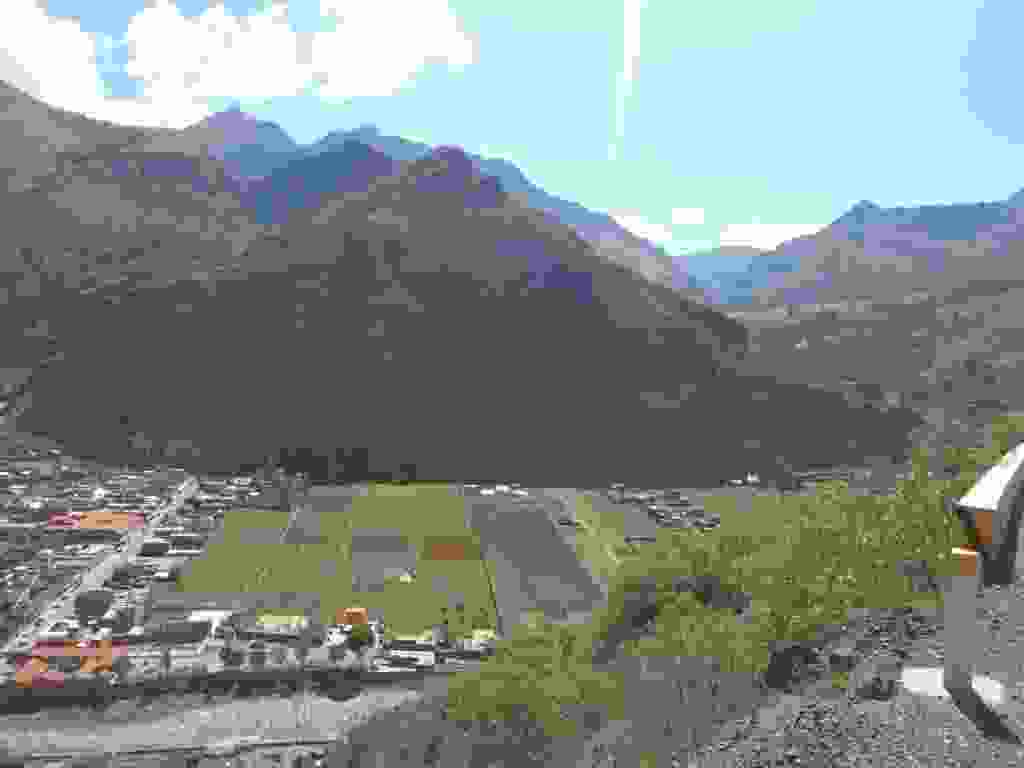
\includegraphics[width=\mywidth]{../wp-content/uploads/2015/05/P5224308-1024x768.jpg} \end{center}
\begin{center} 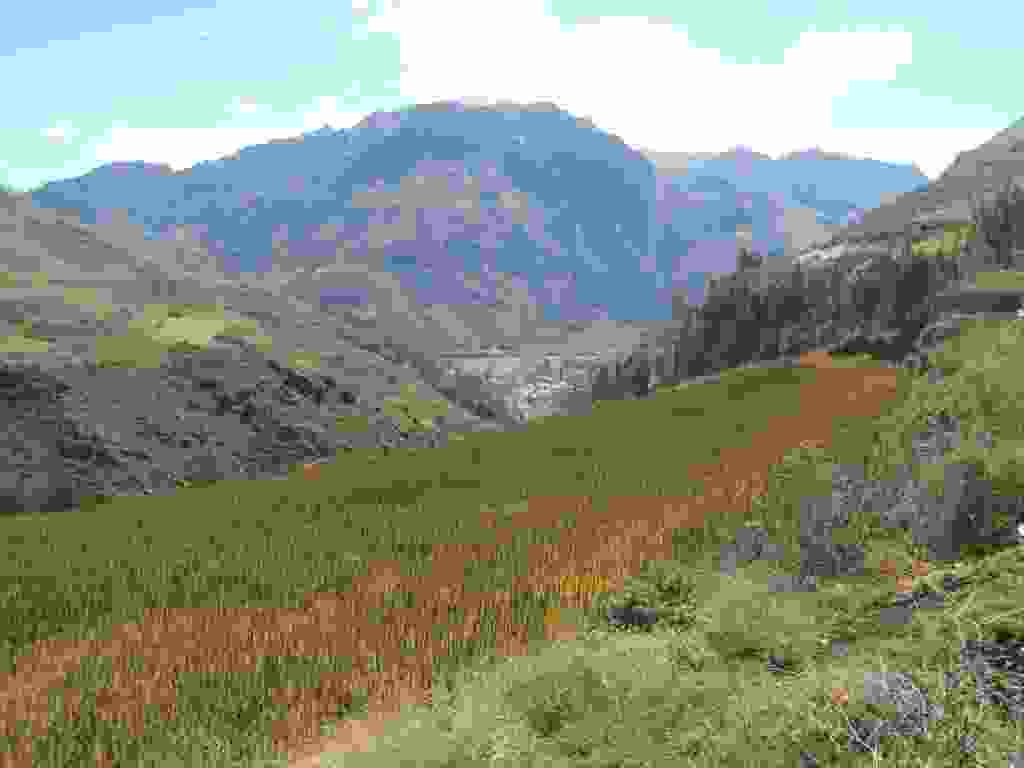
\includegraphics[width=\mywidth]{../wp-content/uploads/2015/05/P5224312-1024x768.jpg} \end{center}

Au milieu de la montée, le sanctuaire des animaux de Cochuahuasi : des lamas, alpagas, vigognes, perroquets, pumas et condors y sont recueillis et soignés. 
\begin{center} 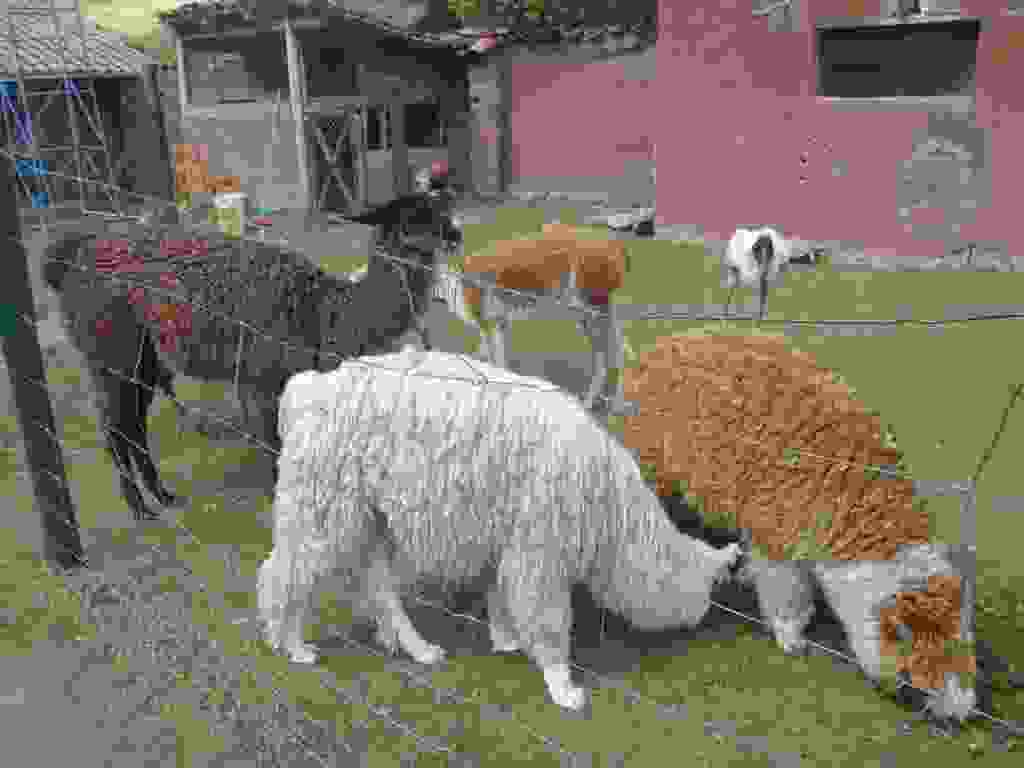
\includegraphics[width=\mywidth]{../wp-content/uploads/2015/05/P5224314-1024x768.jpg} \end{center}
\begin{center} 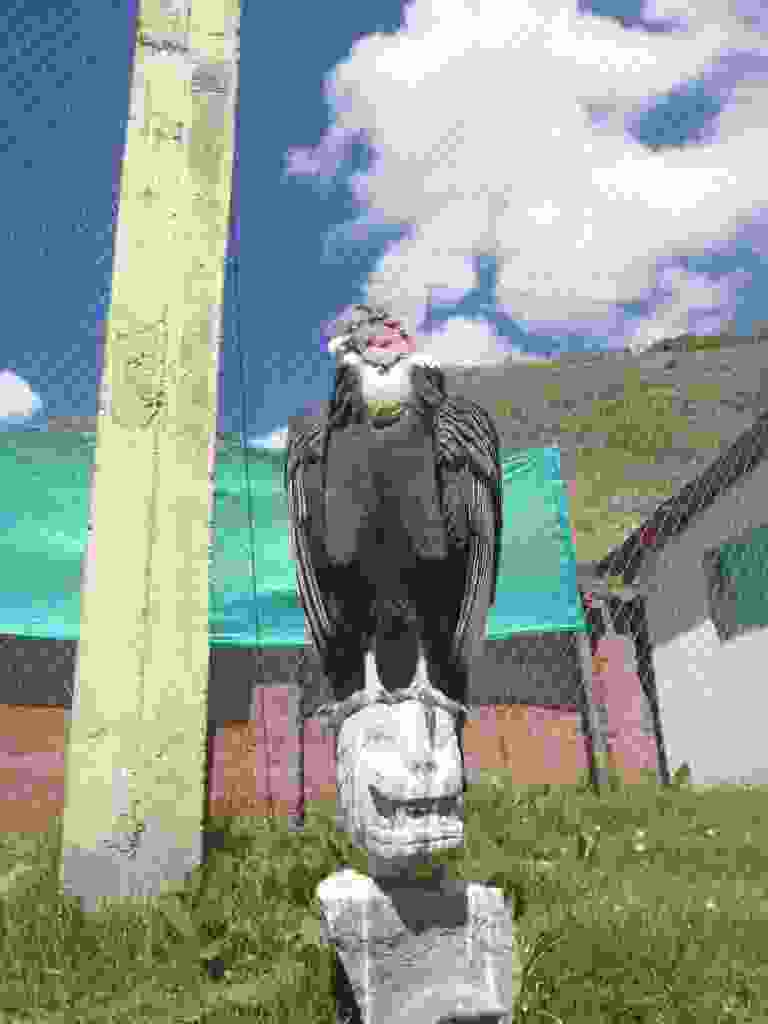
\includegraphics[height=\mywidth]{../wp-content/uploads/2015/05/P5224328-768x1024.jpg} \end{center}
\vfill
\begin{center} \includegraphics[width=\mywidth]{../wp-content/uploads/2015/05/P5224321-1024x768.jpg} \end{center}
\vspace{-\topsep}
\vspace{-0.75mm}